%!TEX root = report.tex

\todo[inline]{Geen grounding -> ballon effect -> add grounding springs. Compare results.}

\todo[inline]{Compare different methods of breaking}

\todo[inline]{Compare different numbers of springs to break per step}


\begin{figure*}
	\centering
	%!TEX root = report.tex	
\begin{subfigure}{0.16\textwidth}
	\centering
	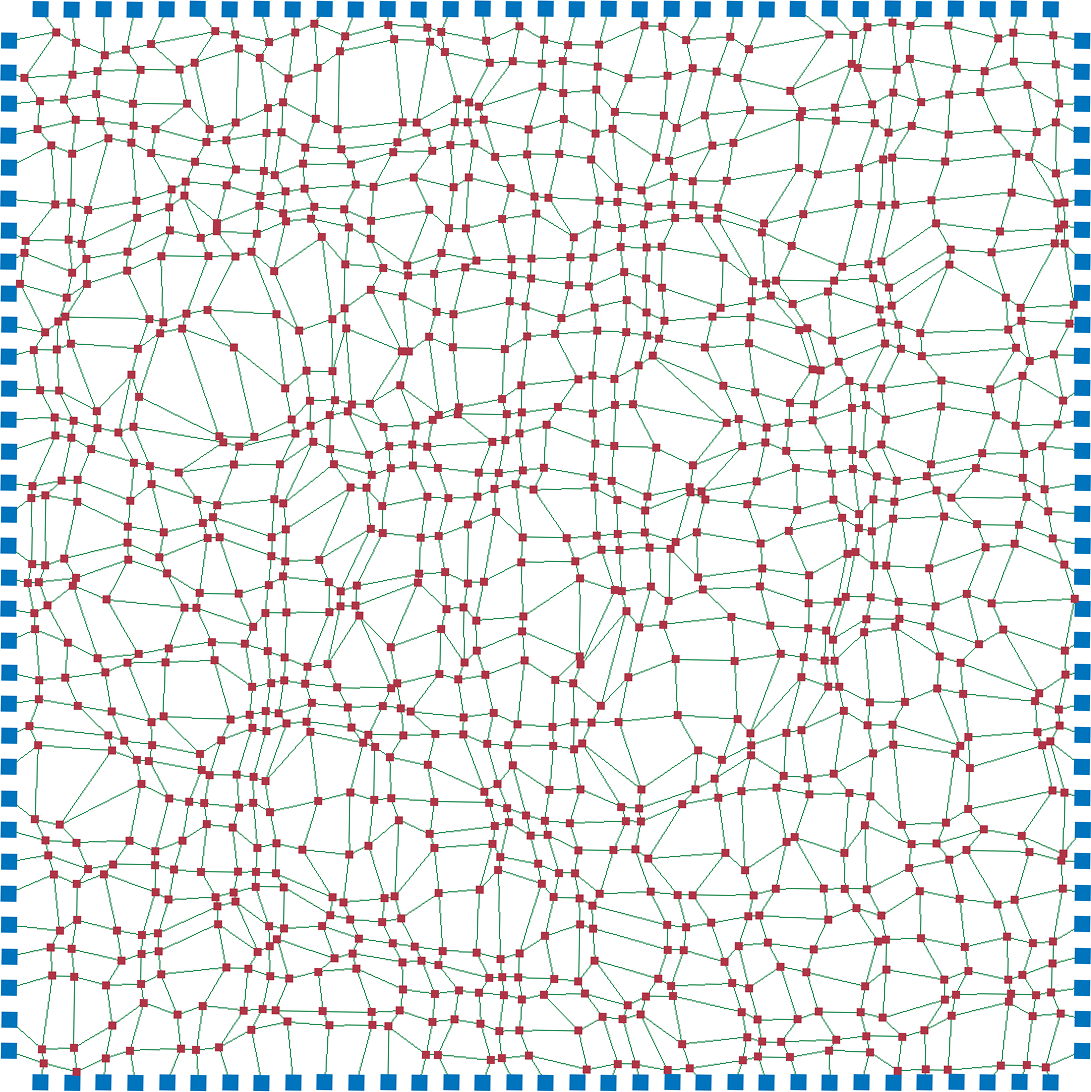
\includegraphics[
		width=\textwidth, 
		height=\textwidth, 
		keepaspectratio=true]
	{./img/results/1200_0_1_highest_97_step_0}
	\caption{Step 0}
	\label{fig:experiment:highestStrain:0}
\end{subfigure}
\begin{subfigure}{0.16\textwidth}
	\centering
	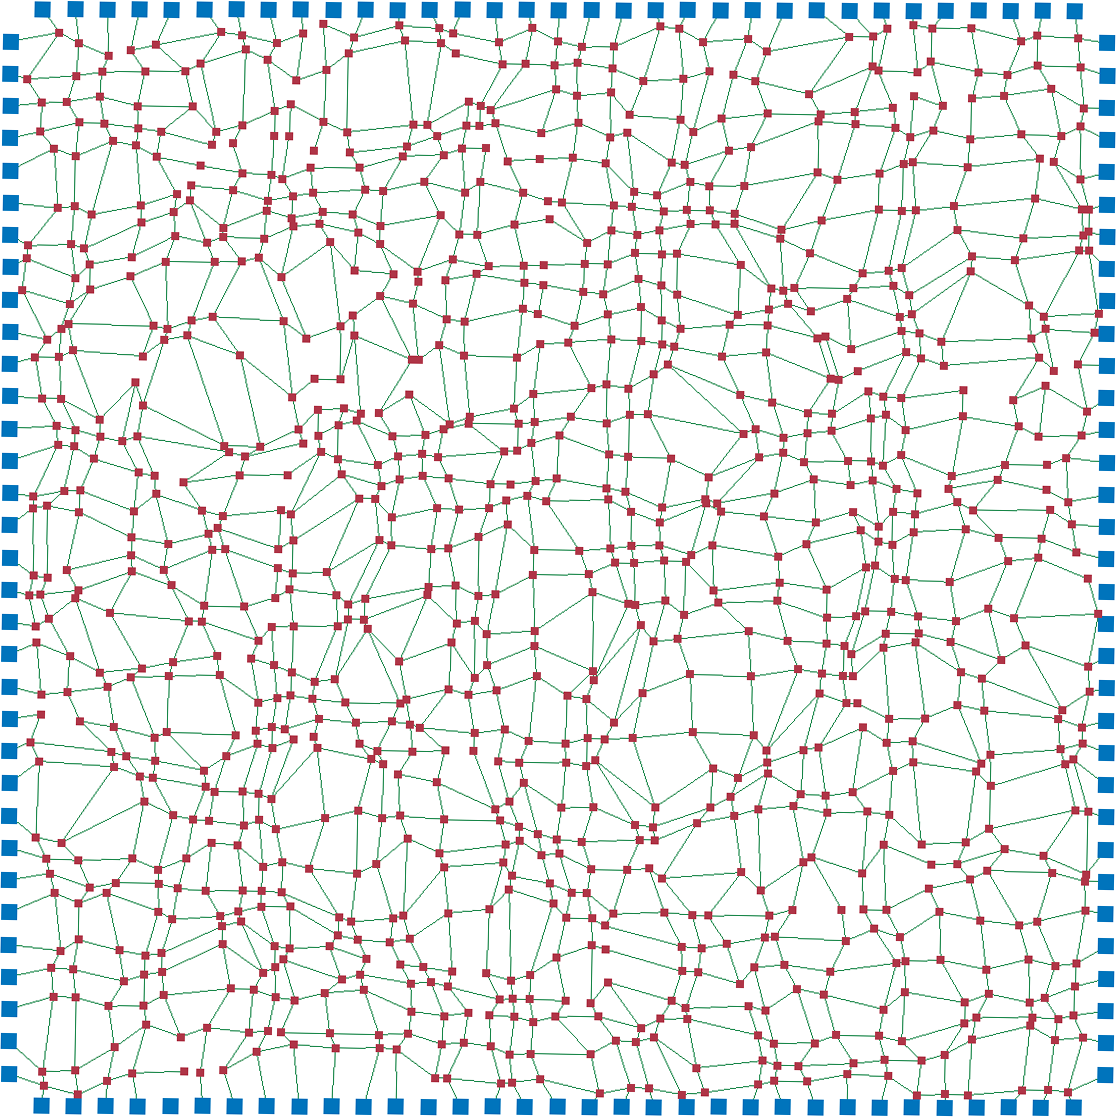
\includegraphics[
		width=\textwidth, 
		height=\textwidth, 
		keepaspectratio=true]
	{./img/results/1200_0_1_highest_97_step_1}
	\caption{Step 1}
	\label{fig:experiment:highestStrain:1}
\end{subfigure}	
\begin{subfigure}{0.16\textwidth}
	\centering
	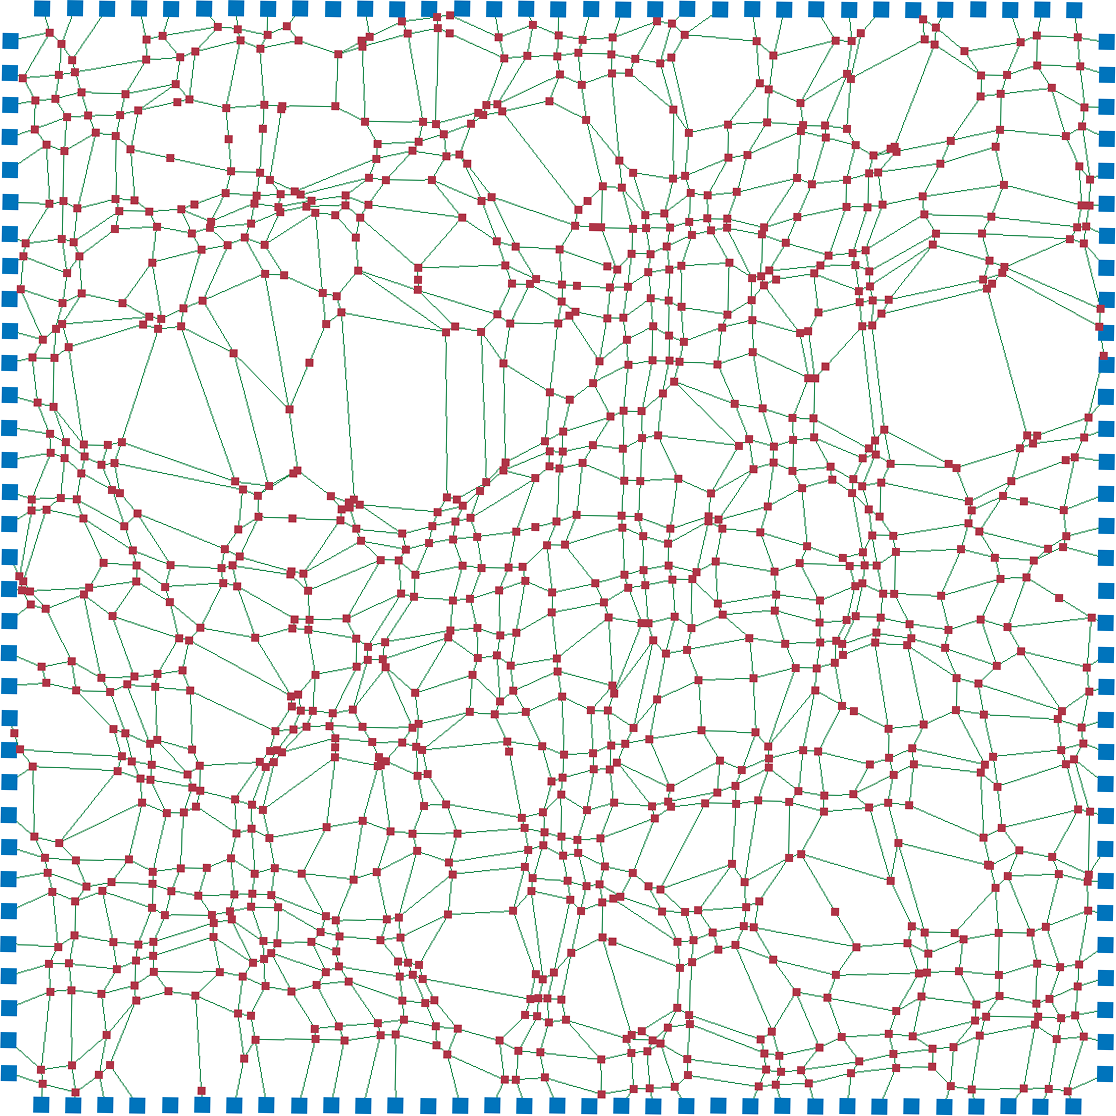
\includegraphics[
		width=\textwidth, 
		height=\textwidth, 
		keepaspectratio=true]
	{./img/results/1200_0_1_highest_97_step_2}
	\caption{Step 2}
	\label{fig:experiment:highestStrain:2}
\end{subfigure}		
\begin{subfigure}{0.16\textwidth}
	\centering
	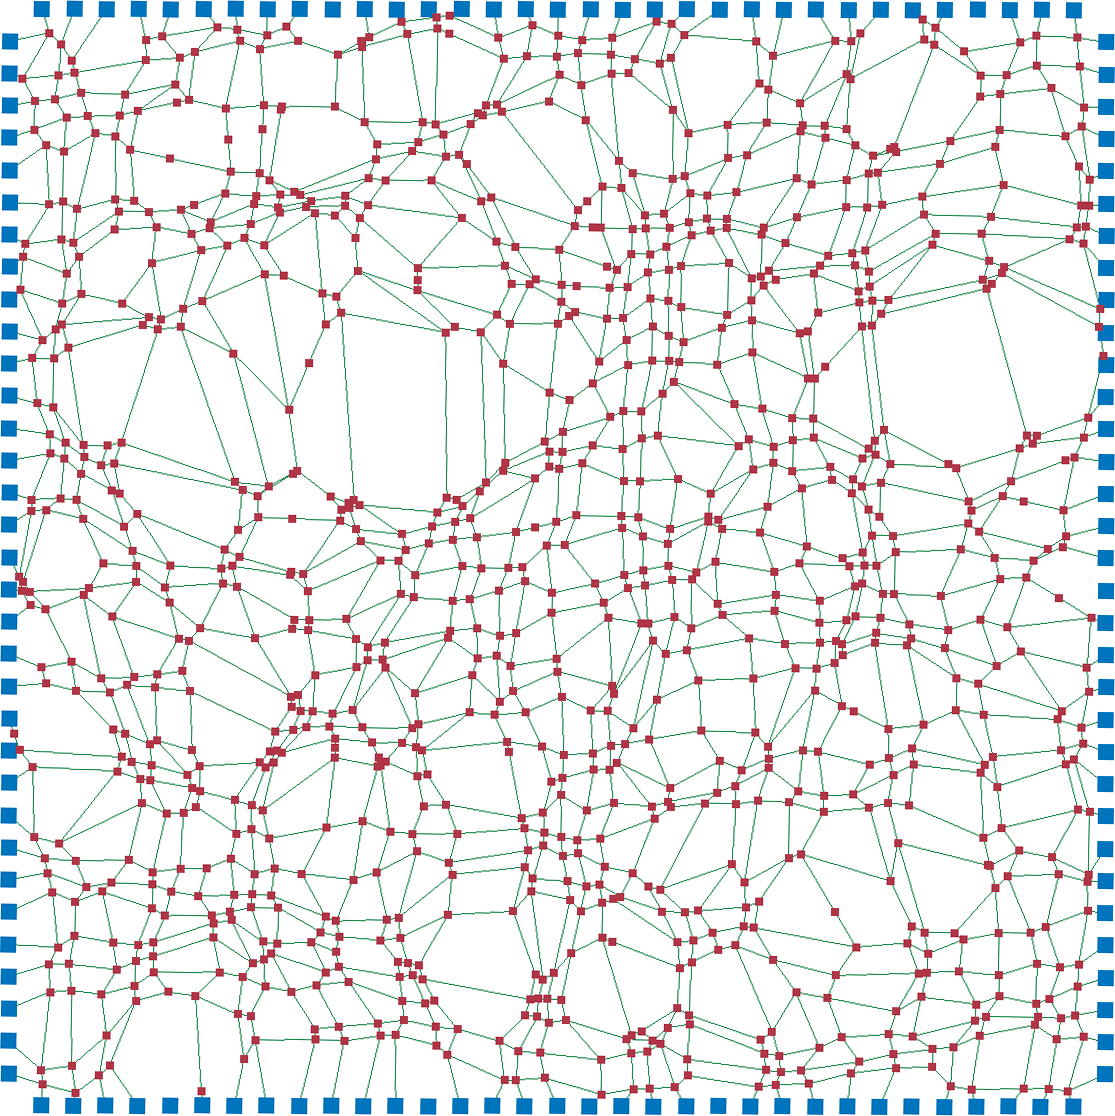
\includegraphics[
		width=\textwidth, 
		height=\textwidth, 
		keepaspectratio=true]
	{./img/results/1200_0_1_highest_97_step_3}
	\caption{Step 3}
	\label{fig:experiment:highestStrain:3}
\end{subfigure}			
\begin{subfigure}{0.16\textwidth}
	\centering
	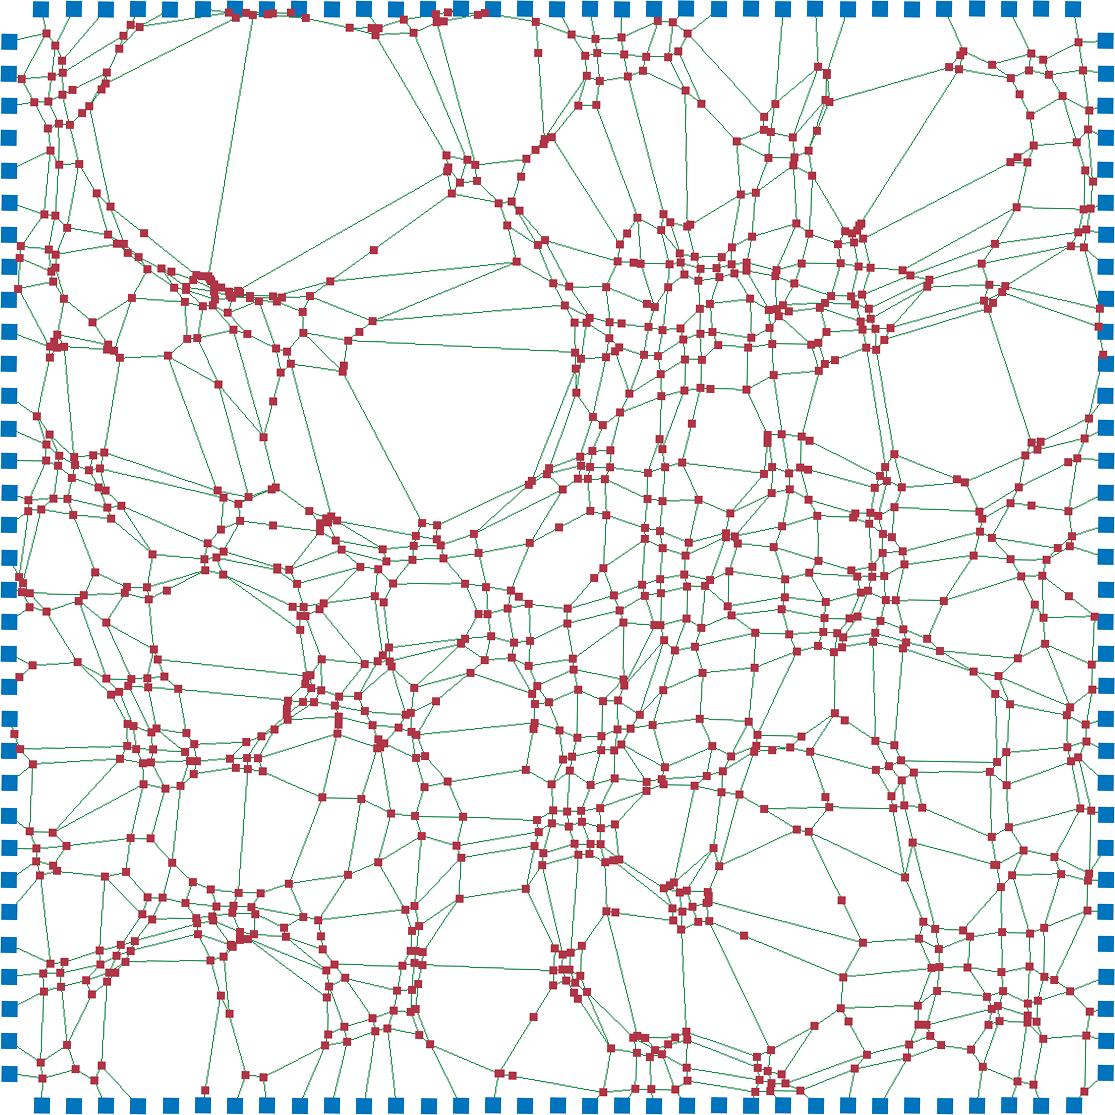
\includegraphics[
		width=\textwidth, 
		height=\textwidth, 
		keepaspectratio=true]
	{./img/results/1200_0_1_highest_97_step_4}
	\caption{Step 4}
	\label{fig:experiment:highestStrain:4}
\end{subfigure}				
\begin{subfigure}{0.16\textwidth}
	\centering
	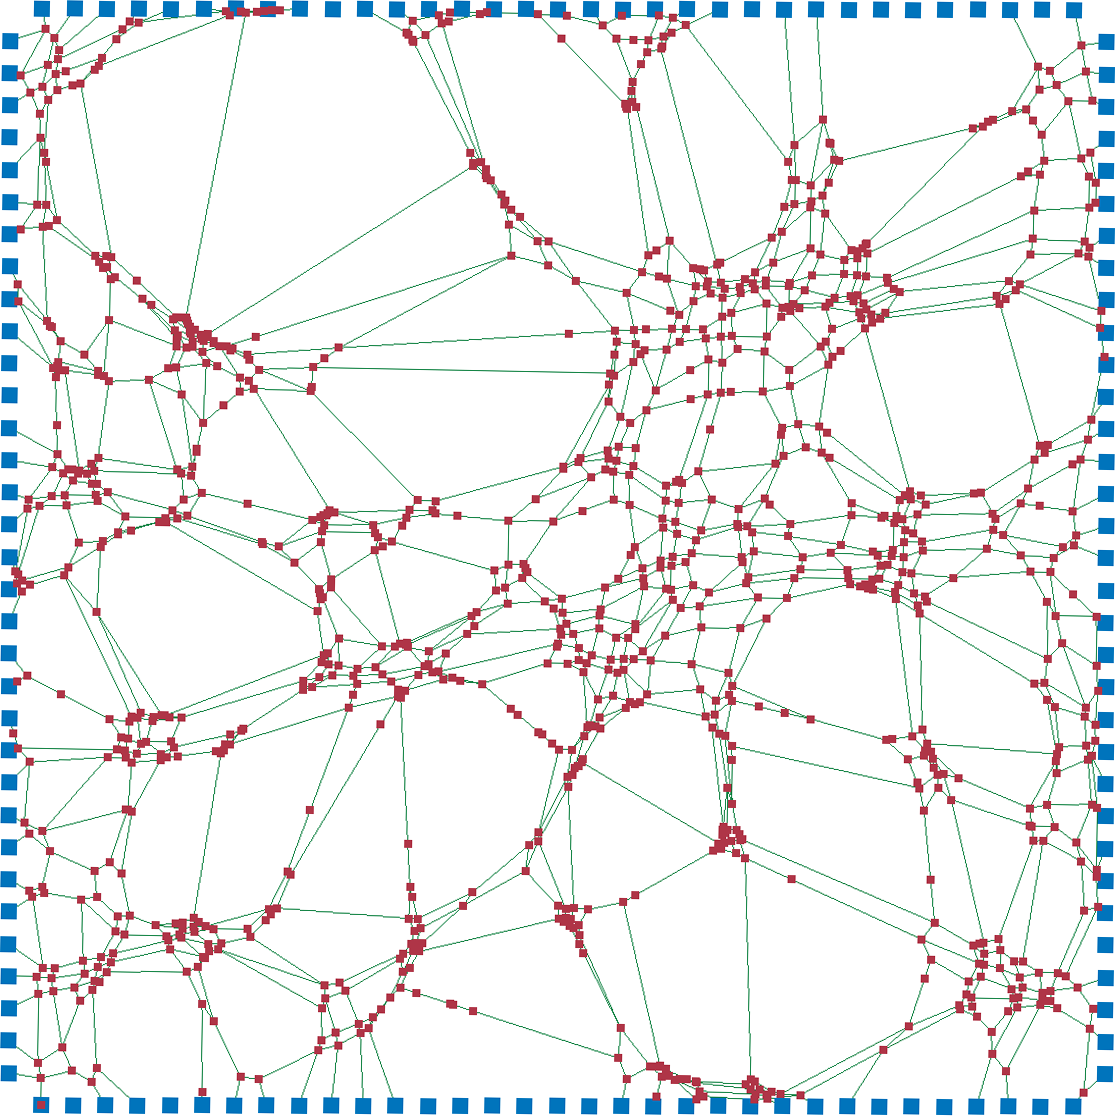
\includegraphics[
		width=\textwidth, 
		height=\textwidth, 
		keepaspectratio=true]
	{./img/results/1200_0_1_highest_97_step_5}
	\caption{Step 5}
	\label{fig:experiment:highestStrain:5}
\end{subfigure}
\begin{subfigure}{0.16\textwidth}
	\centering
	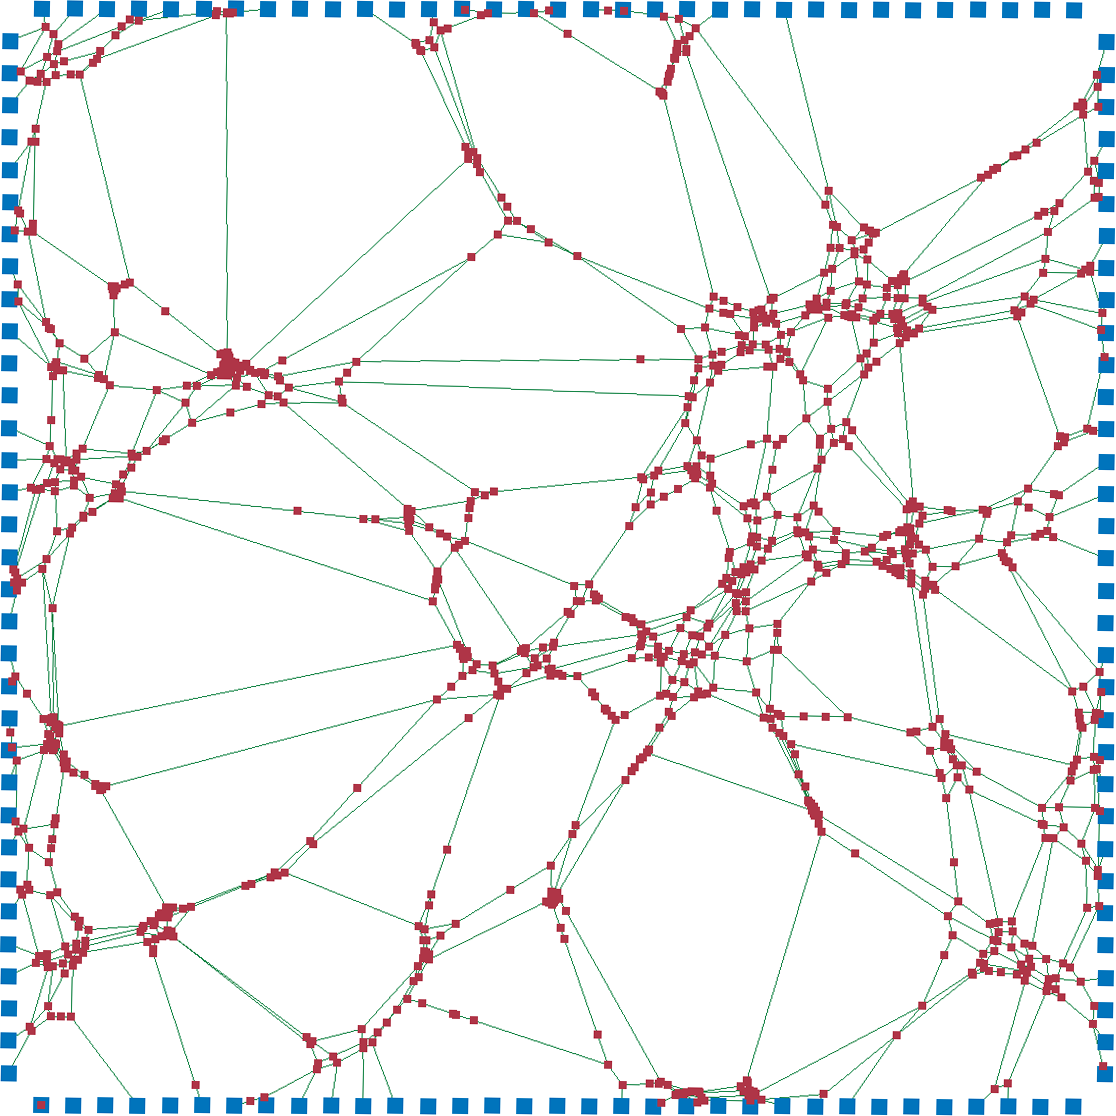
\includegraphics[
		width=\textwidth, 
		height=\textwidth, 
		keepaspectratio=true]
	{./img/results/1200_0_1_highest_97_step_6}
	\caption{Step 6}
	\label{fig:experiment:highestStrain:6}
\end{subfigure}	
\begin{subfigure}{0.16\textwidth}
	\centering
	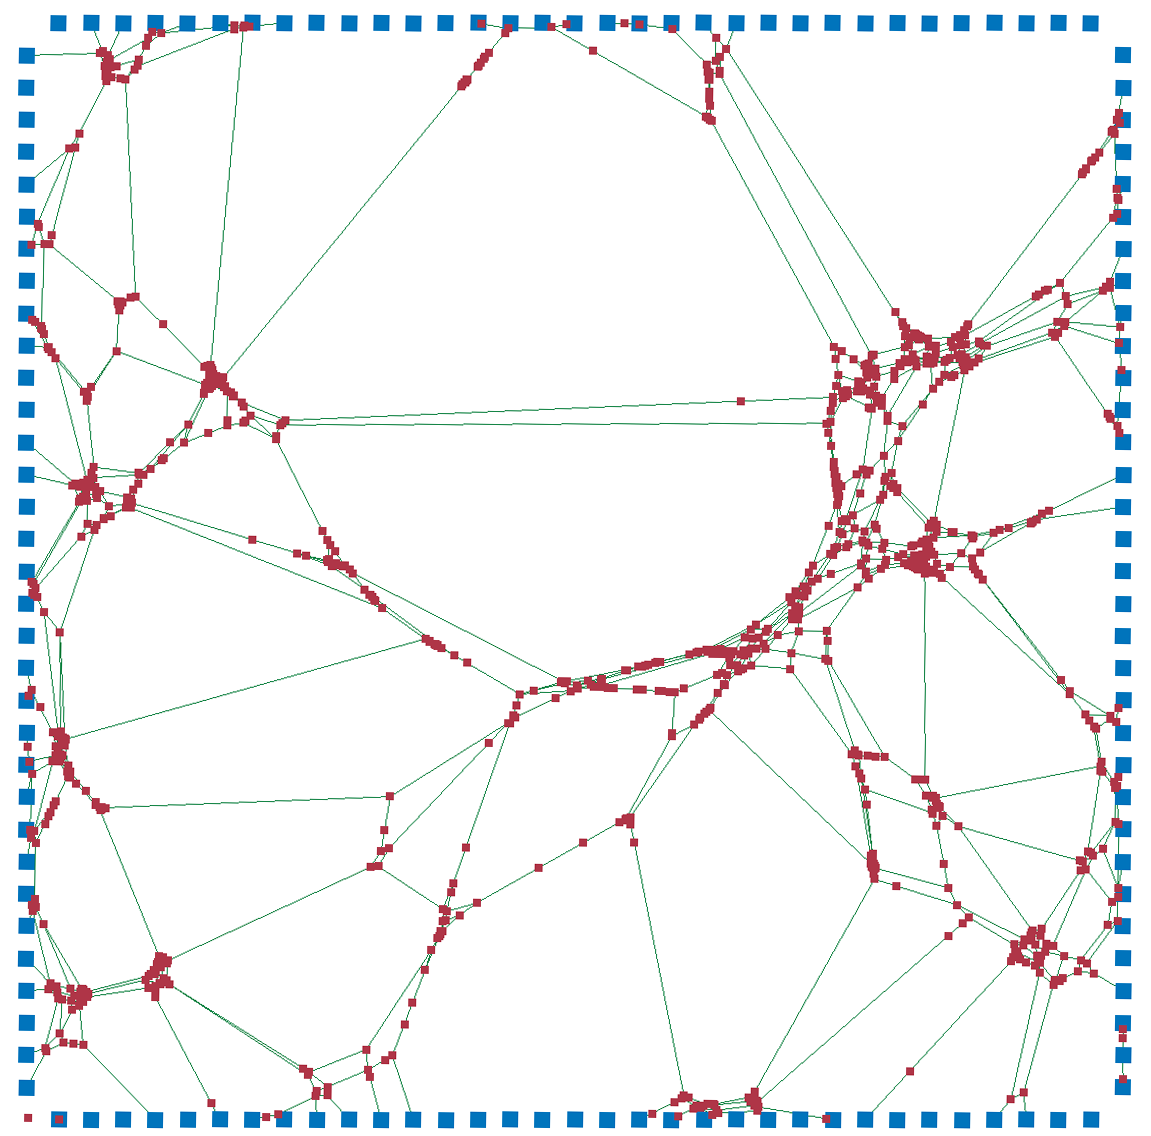
\includegraphics[
		width=\textwidth, 
		height=\textwidth, 
		keepaspectratio=true]
	{./img/results/1200_0_1_highest_97_step_7}
	\caption{Step 7}
	\label{fig:experiment:highestStrain:7}
\end{subfigure}		
\begin{subfigure}{0.16\textwidth}
	\centering
	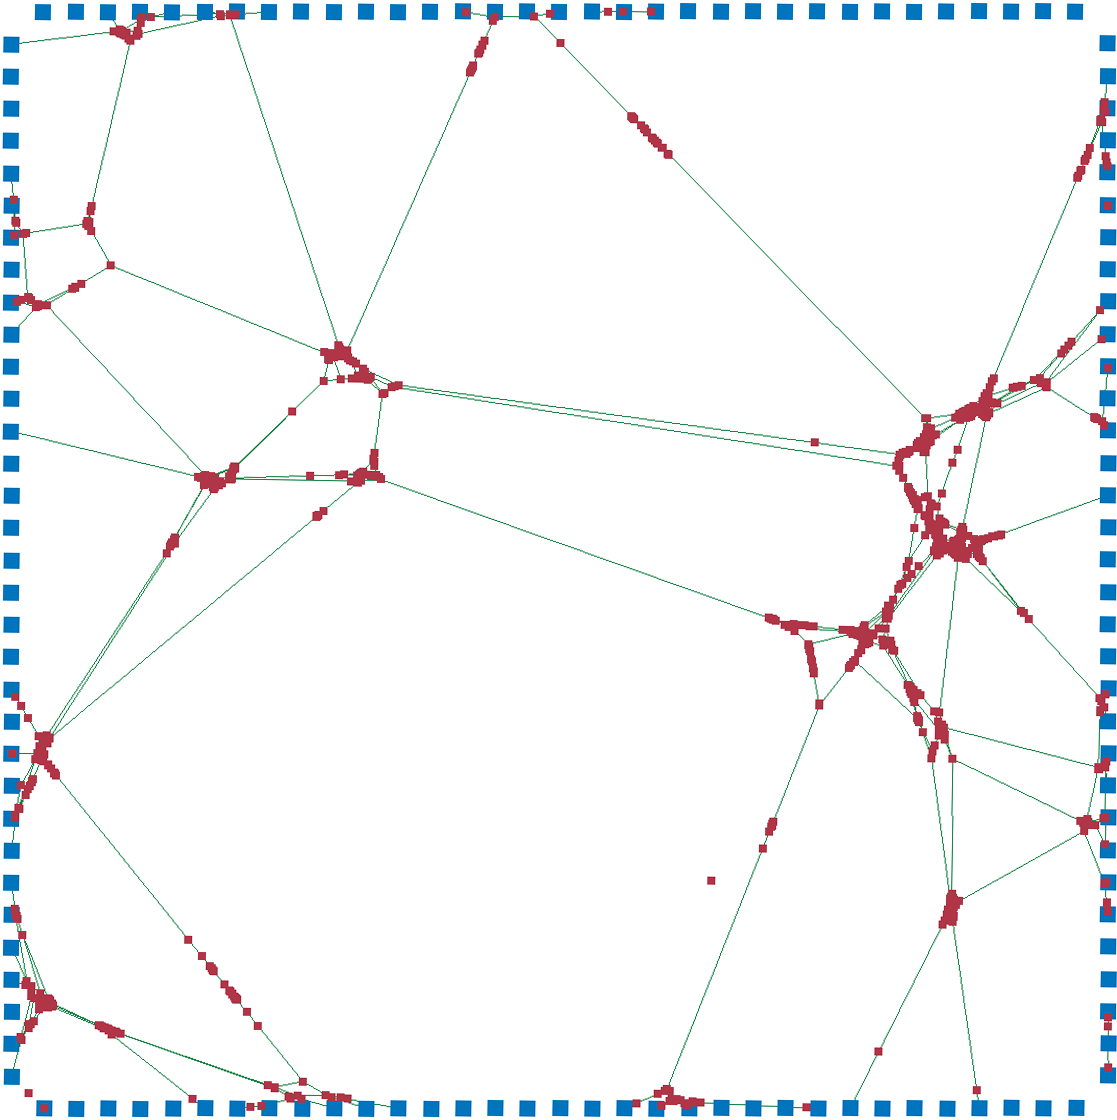
\includegraphics[
		width=\textwidth, 
		height=\textwidth, 
		keepaspectratio=true]
	{./img/results/1200_0_1_highest_97_step_8}
	\caption{Step 8}
	\label{fig:experiment:highestStrain:8}
\end{subfigure}			
\begin{subfigure}{0.16\textwidth}
	\centering
	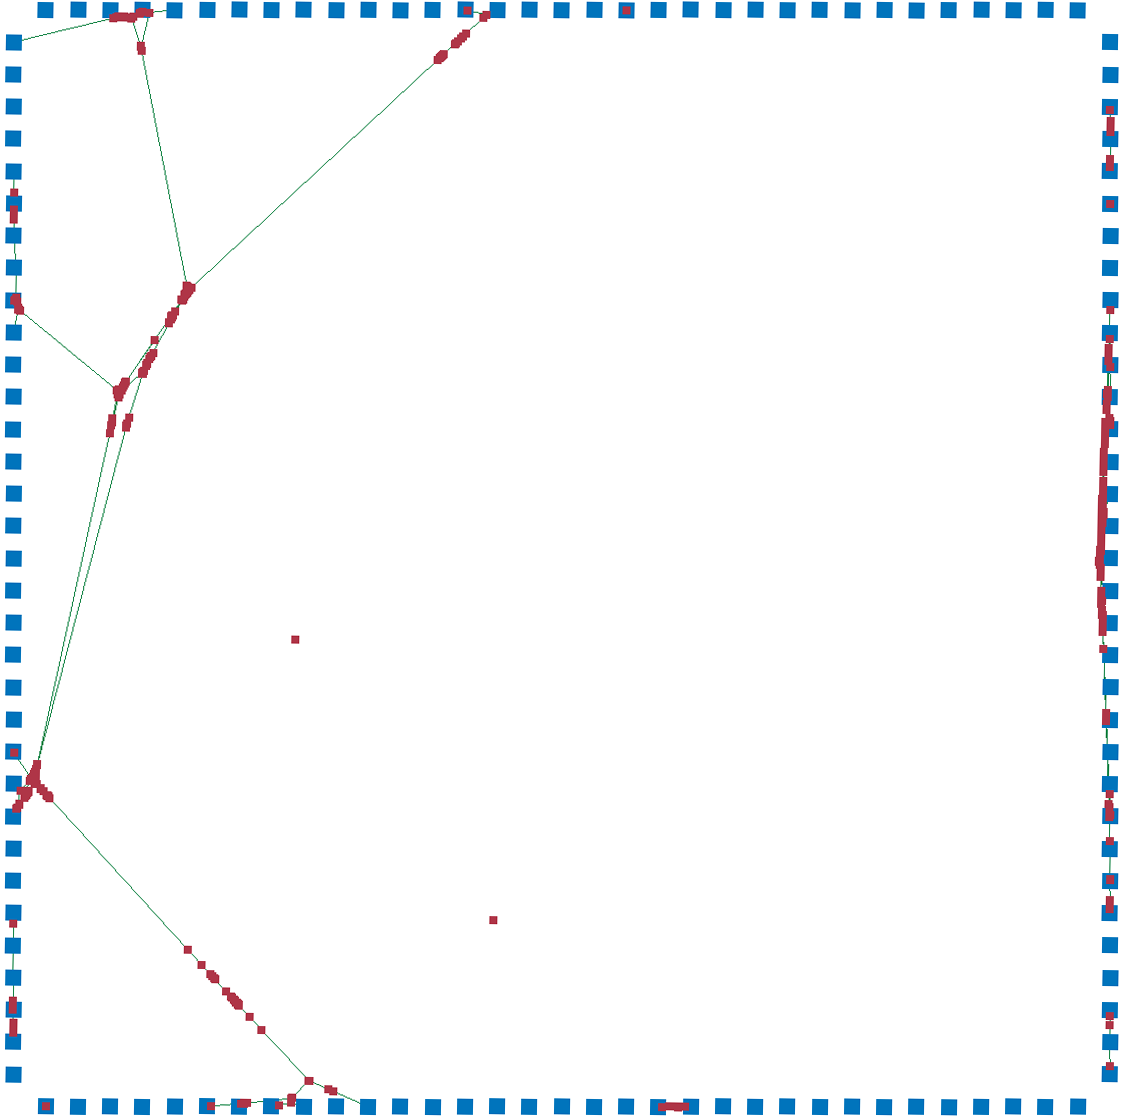
\includegraphics[
		width=\textwidth, 
		height=\textwidth, 
		keepaspectratio=true]
	{./img/results/1200_0_1_highest_97_step_9}
	\caption{Step 9}
	\label{fig:experiment:highestStrain:9}
\end{subfigure}					
\begin{subfigure}{0.16\textwidth}
	\centering
	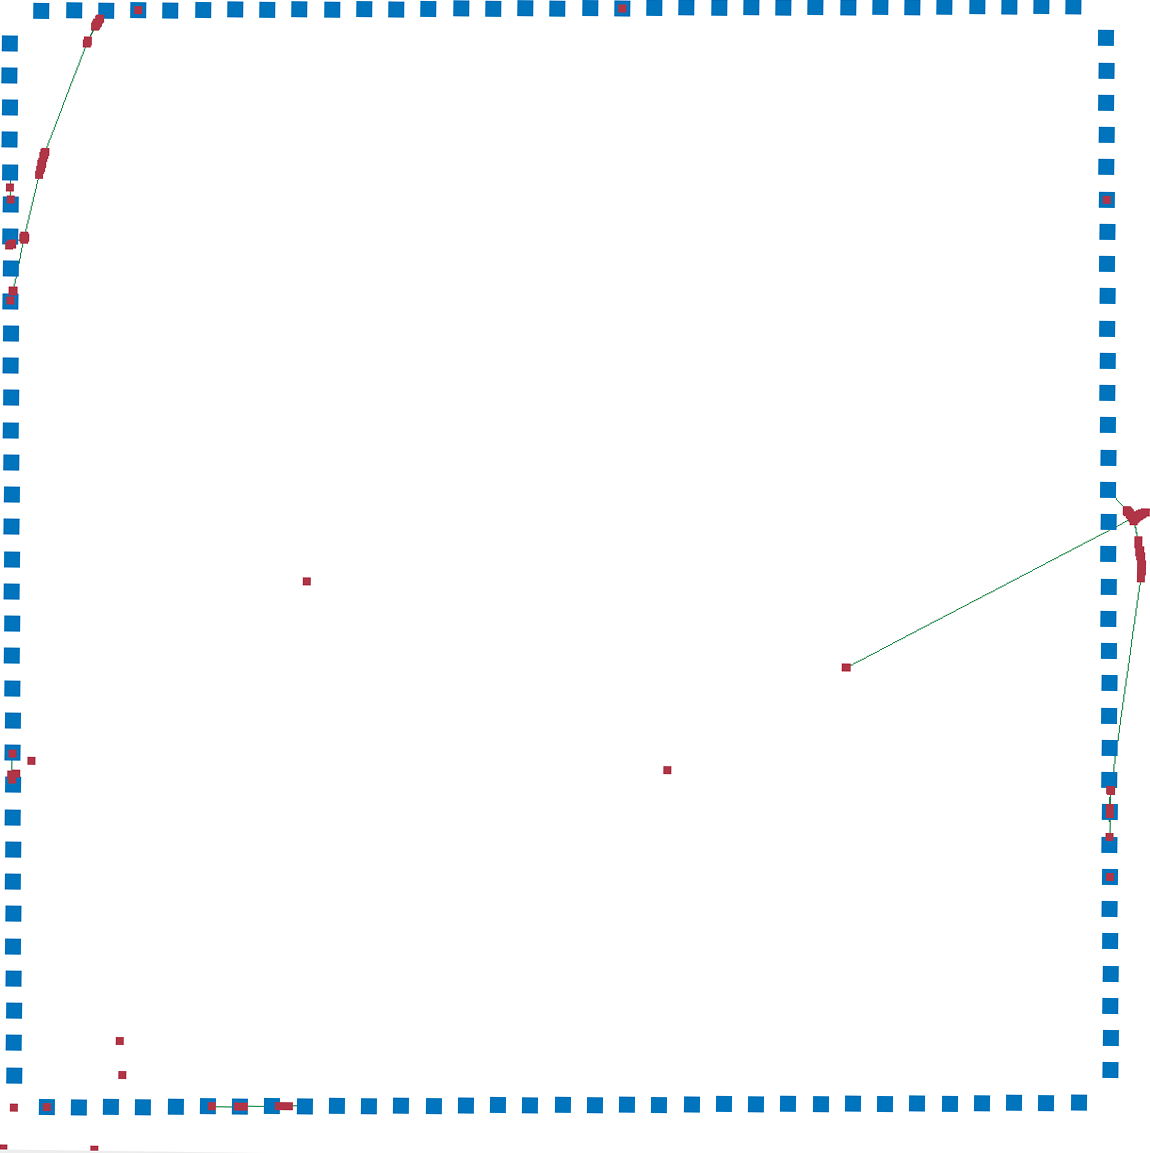
\includegraphics[
		width=\textwidth, 
		height=\textwidth, 
		keepaspectratio=true]
	{./img/results/1200_0_1_highest_97_step_10}
	\caption{Step 10}
	\label{fig:experiment:highestStrain:10}
\end{subfigure}			
\begin{subfigure}{0.16\textwidth}
	\centering
	
\includegraphics[
		width=\textwidth, 
		height=\textwidth, 
		keepaspectratio=true]
	{./img/results/1200_0_1_highest_97_step_11}
	\caption{Step 11}
	\label{fig:experiment:highestStrain:11}
\end{subfigure}						
	\caption{Several steps of the breaking of springs, where the 97 springs with the highest strain were broken. The grid had 1200 particles, the spring constants were sampled from a normal distribution with mean 0.0 and standard deviation 1.0. Step 0 is a stabilization of the initial grid, presented in \cref{fig:implementation:stabilizedInitial}, the following steps are the stabilization and breaking steps of the algorithm.}
	\label{fig:experiment:highestStrain}
\end{figure*}

\begin{figure*}
	\centering
	%!TEX root = report.tex	
\begin{subfigure}{0.16\textwidth}
	\centering
	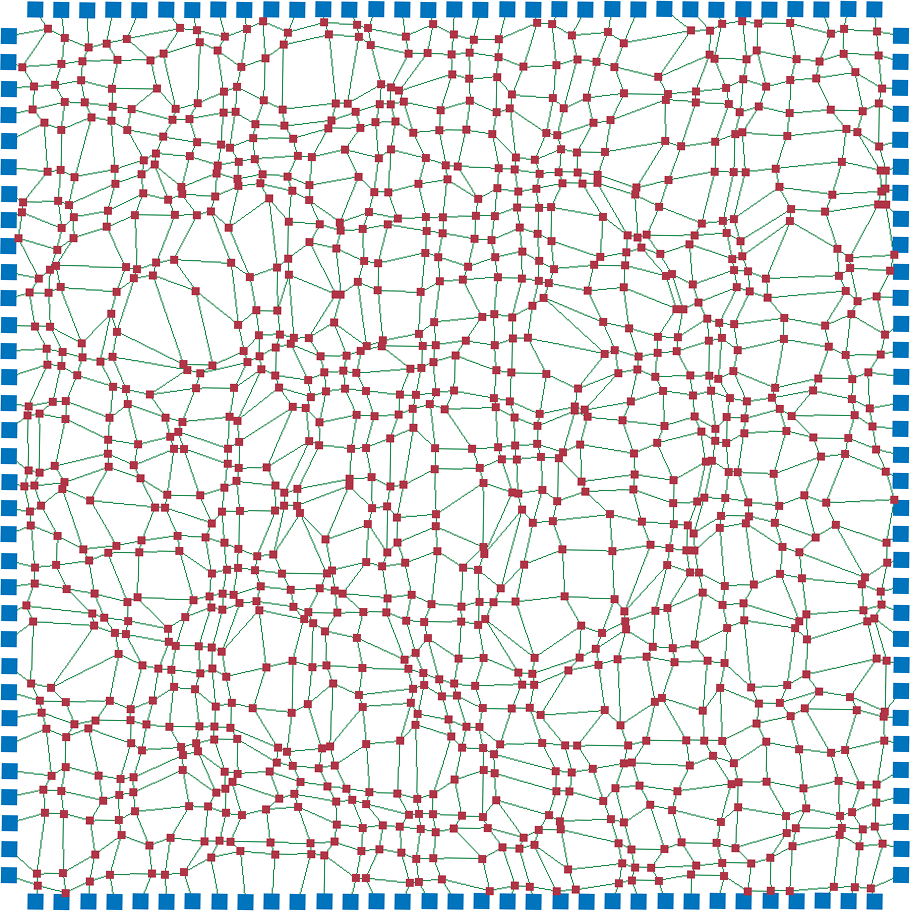
\includegraphics[
		width=\textwidth, 
		height=\textwidth, 
		keepaspectratio=true]
	{./img/results/1200_0_1_greater_104_step_0}
	\caption{}
	\label{fig:experiment:greaterThanStrain:0}
\end{subfigure}
\begin{subfigure}{0.16\textwidth}
	\centering
	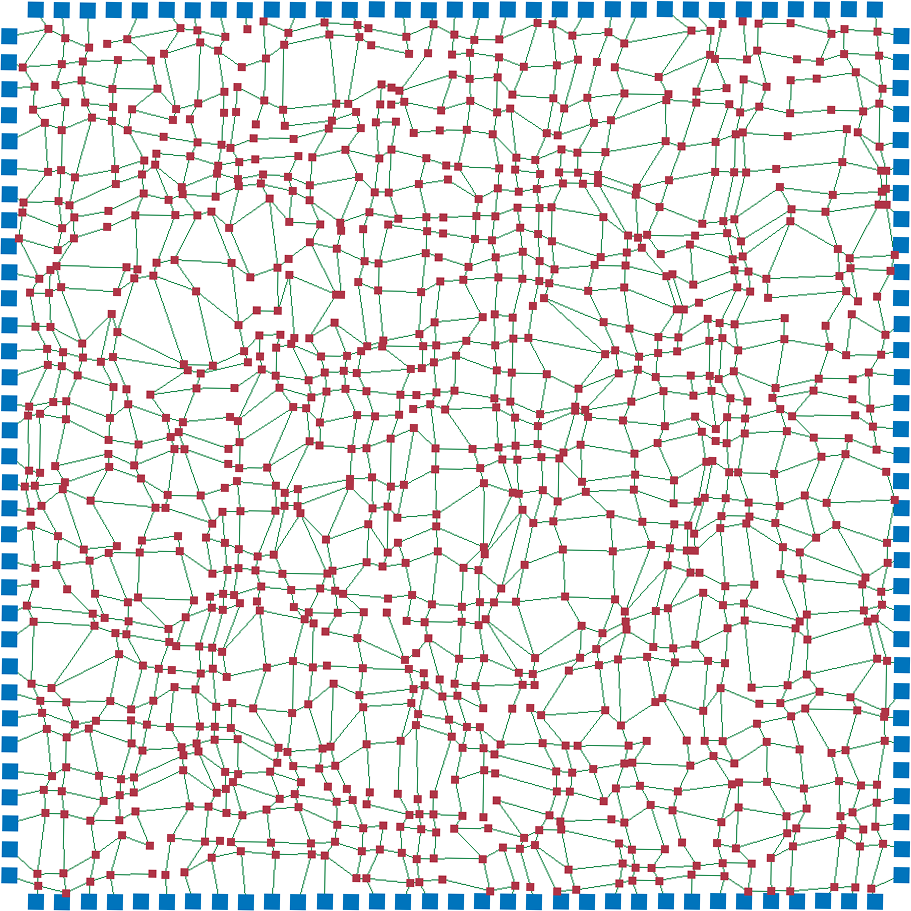
\includegraphics[
		width=\textwidth, 
		height=\textwidth, 
		keepaspectratio=true]
	{./img/results/1200_0_1_greater_104_step_1}
	\caption{}
	\label{fig:experiment:greaterThanStrain:1}
\end{subfigure}	
\begin{subfigure}{0.16\textwidth}
	\centering
	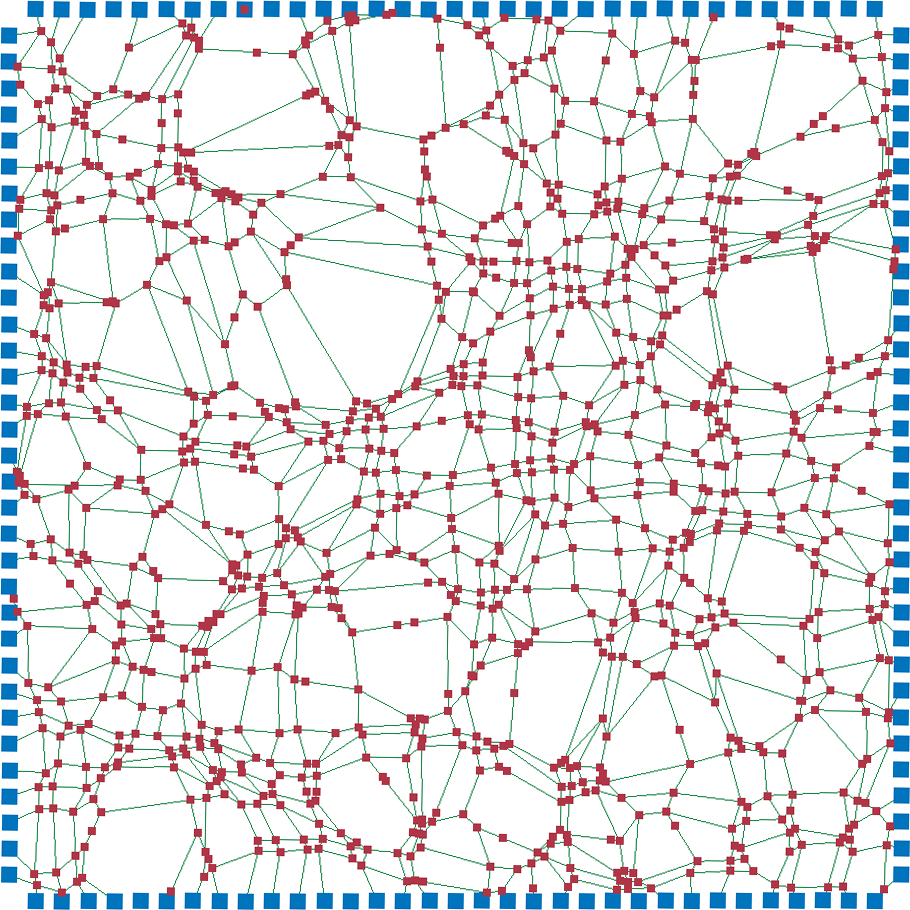
\includegraphics[
		width=\textwidth, 
		height=\textwidth, 
		keepaspectratio=true]
	{./img/results/1200_0_1_greater_104_step_2}
	\caption{}
	\label{fig:experiment:greaterThanStrain:2}
\end{subfigure}		
\begin{subfigure}{0.16\textwidth}
	\centering
	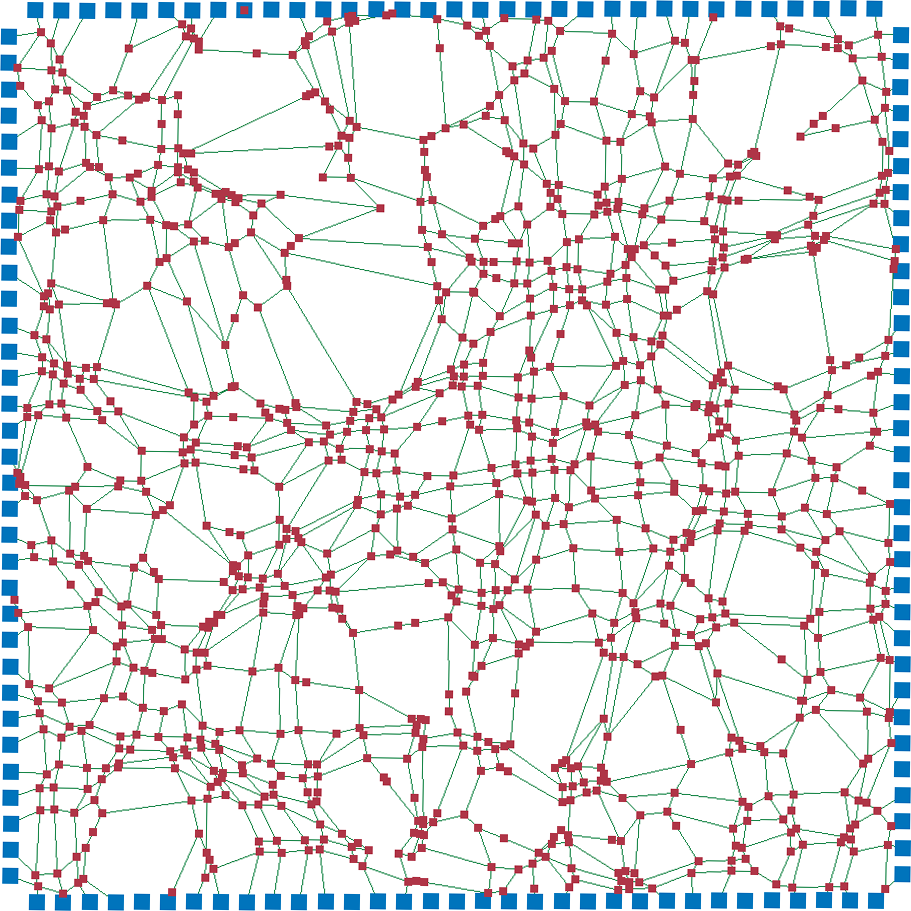
\includegraphics[
		width=\textwidth, 
		height=\textwidth, 
		keepaspectratio=true]
	{./img/results/1200_0_1_greater_104_step_3}
	\caption{}
	\label{fig:experiment:greaterThanStrain:3}
\end{subfigure}			

\begin{subfigure}{0.16\textwidth}
	\centering
	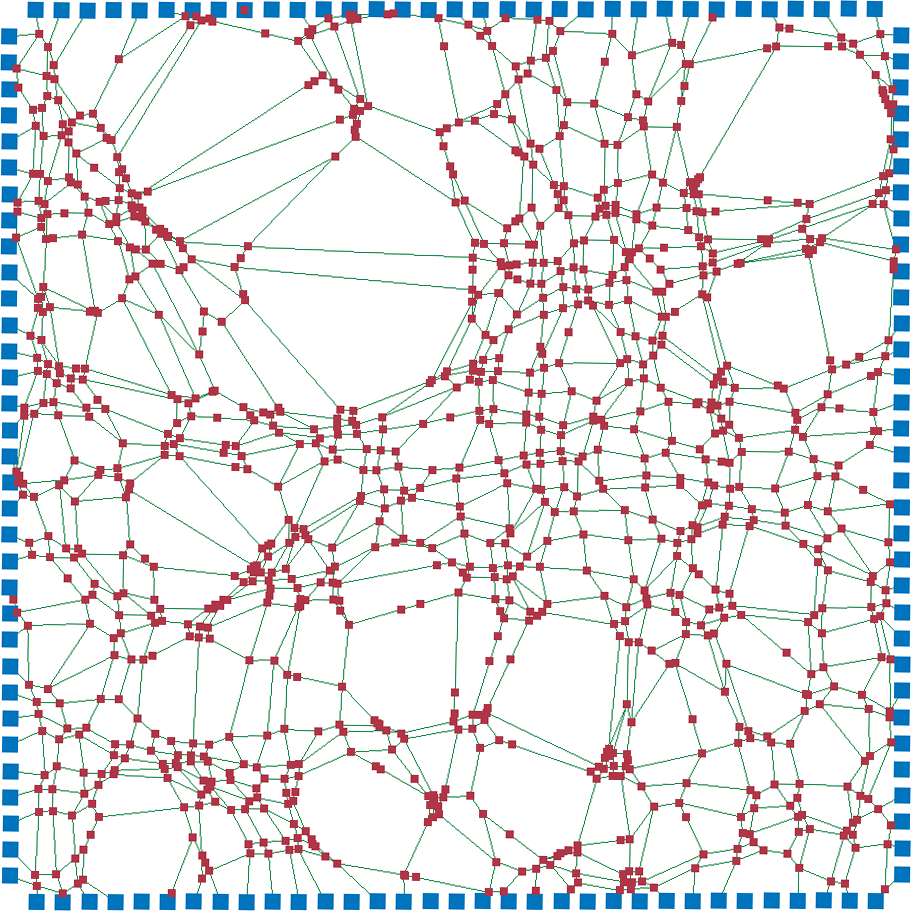
\includegraphics[
		width=\textwidth, 
		height=\textwidth, 
		keepaspectratio=true]
	{./img/results/1200_0_1_greater_104_step_4}
	\caption{}
	\label{fig:experiment:greaterThanStrain:4}
\end{subfigure}				
\begin{subfigure}{0.16\textwidth}
	\centering
	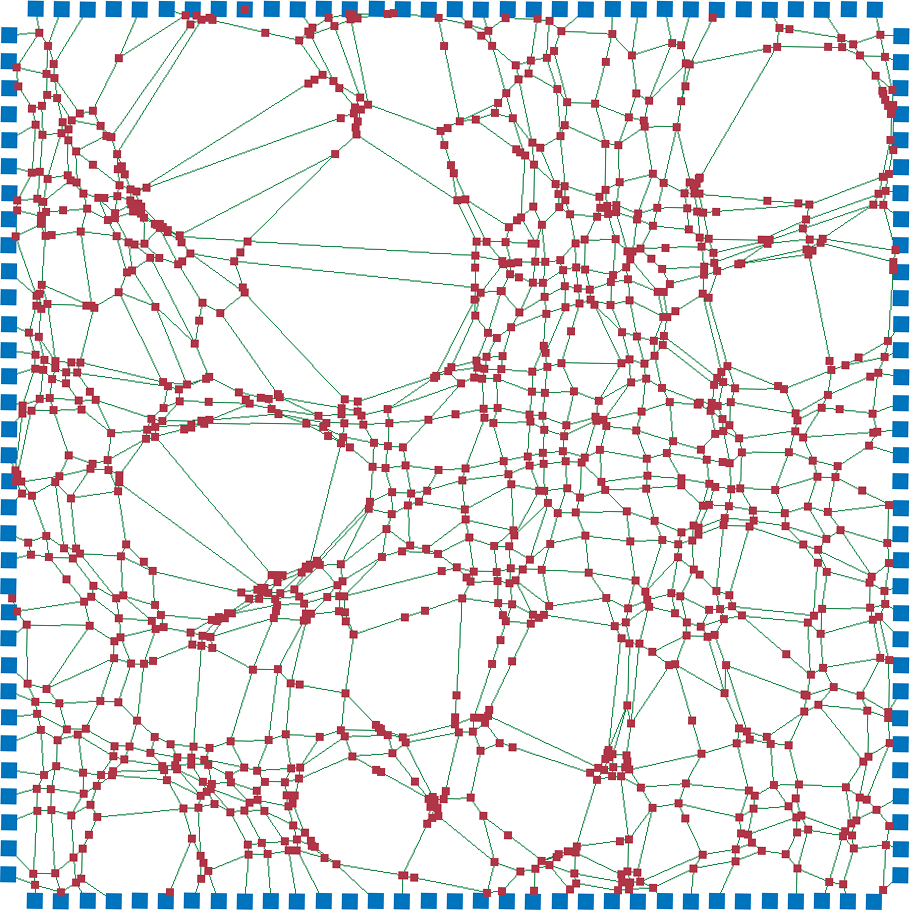
\includegraphics[
		width=\textwidth, 
		height=\textwidth, 
		keepaspectratio=true]
	{./img/results/1200_0_1_greater_104_step_5}
	\caption{}
	\label{fig:experiment:greaterThanStrain:5}
\end{subfigure}
\begin{subfigure}{0.16\textwidth}
	\centering
	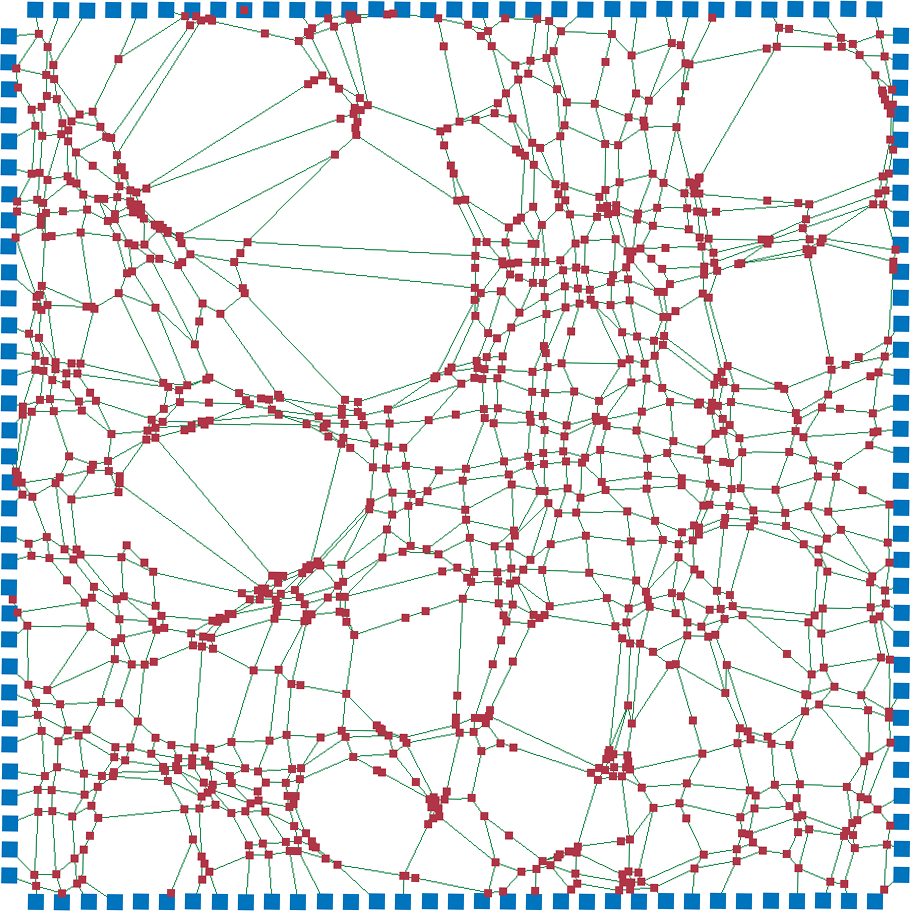
\includegraphics[
		width=\textwidth, 
		height=\textwidth, 
		keepaspectratio=true]
	{./img/results/1200_0_1_greater_104_step_6}
	\caption{}
	\label{fig:experiment:greaterThanStrain:6}
\end{subfigure}	
\begin{subfigure}{0.16\textwidth}
	\centering
	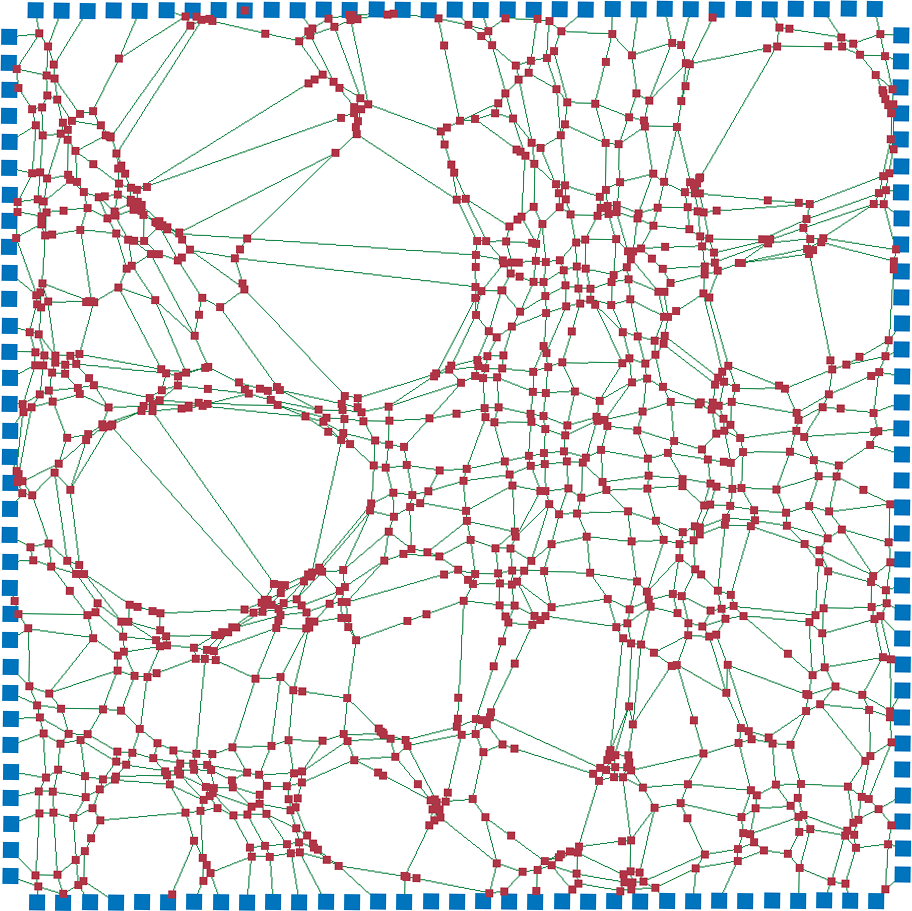
\includegraphics[
		width=\textwidth, 
		height=\textwidth, 
		keepaspectratio=true]
	{./img/results/1200_0_1_greater_104_step_7}
	\caption{}
	\label{fig:experiment:greaterThanStrain:7}
\end{subfigure}							
	\caption{Several steps of the breaking of springs, where the springs with a strain greater than 1.04 were broken. The grid had 1200 particles, the spring constants were sampled from a normal distribution with mean 0.0 and standard deviation 1.0. Step 0 is a stabilization of the initial grid, presented in \cref{fig:implementation:stabilizedInitial}, the following steps are the stabilization and breaking steps of the algorithm.}
	\label{fig:experiment:greaterThanStrain}
\end{figure*}

\begin{figure*}
	\centering
	%!TEX root = report.tex	
\begin{subfigure}{0.16\textwidth}
	\centering
	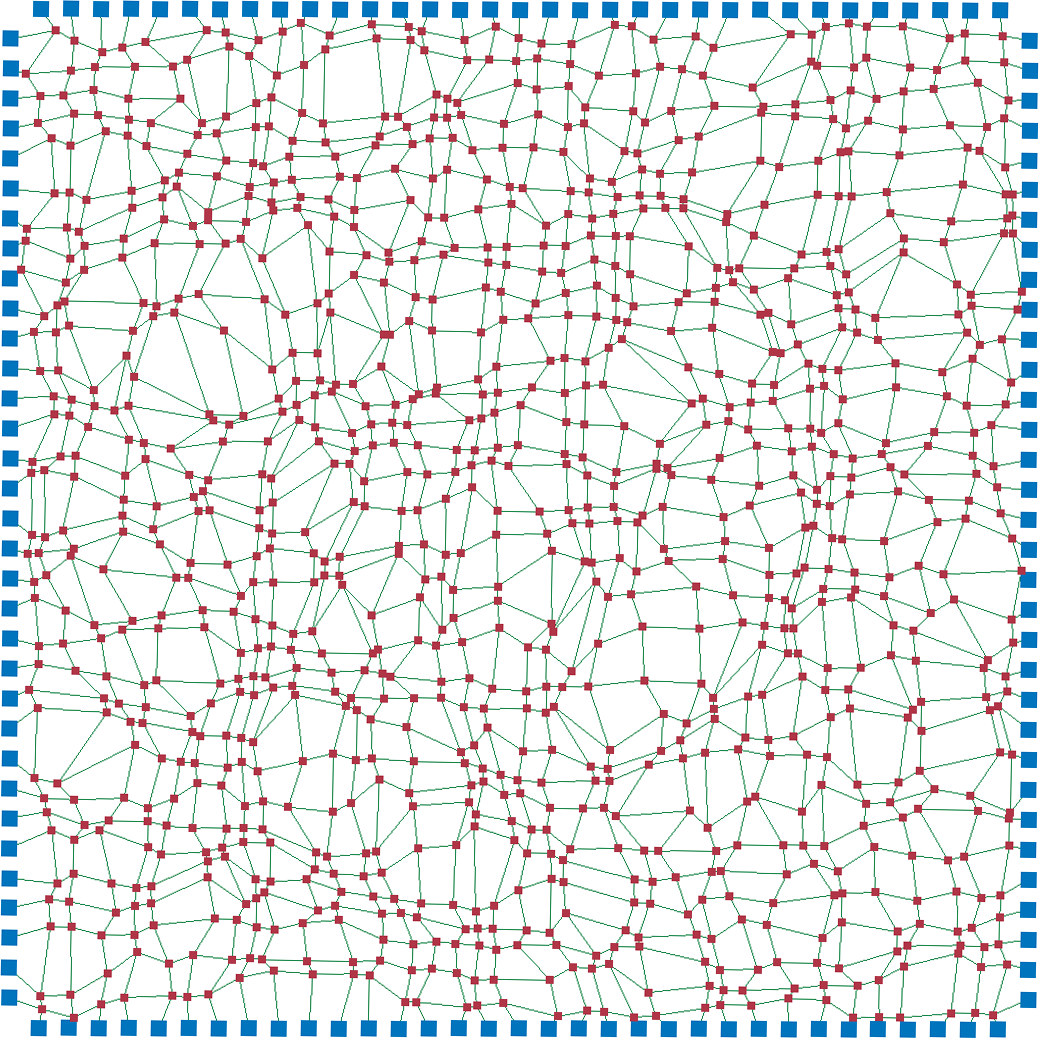
\includegraphics[
		width=\textwidth, 
		height=\textwidth, 
		keepaspectratio=true]
	{./img/results/1200_0_1_stretchGreaterThan_104_step_1}
	%\caption{Step 0}
	%\label{fig:experiment:stretchGreaterThanStrain:1}
\end{subfigure}	
\begin{subfigure}{0.16\textwidth}
	\centering
	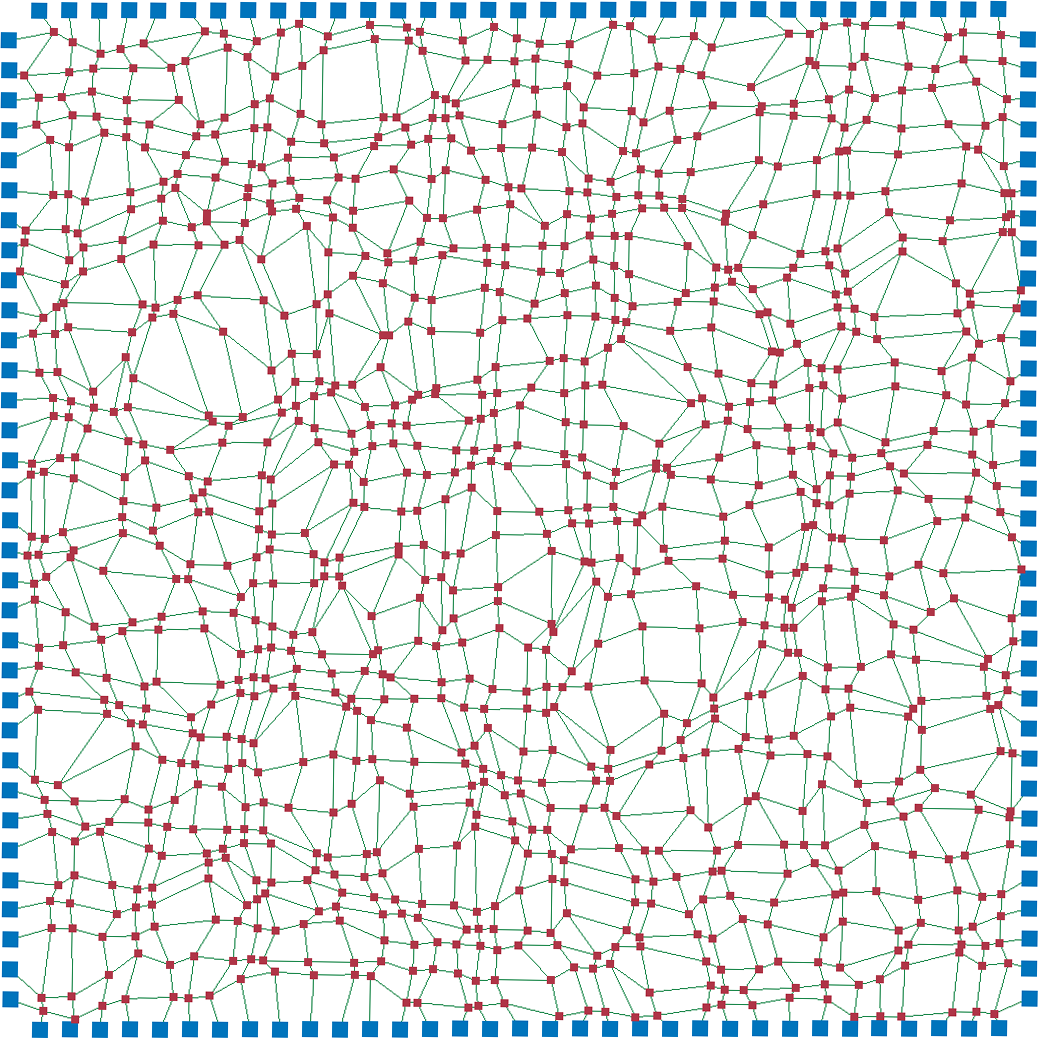
\includegraphics[
		width=\textwidth, 
		height=\textwidth, 
		keepaspectratio=true]
	{./img/results/1200_0_1_stretchGreaterThan_104_step_2}
	%\caption{Step 1}
	%\label{fig:experiment:stretchGreaterThanStrain:2}
\end{subfigure}		
\begin{subfigure}{0.16\textwidth}
	\centering
	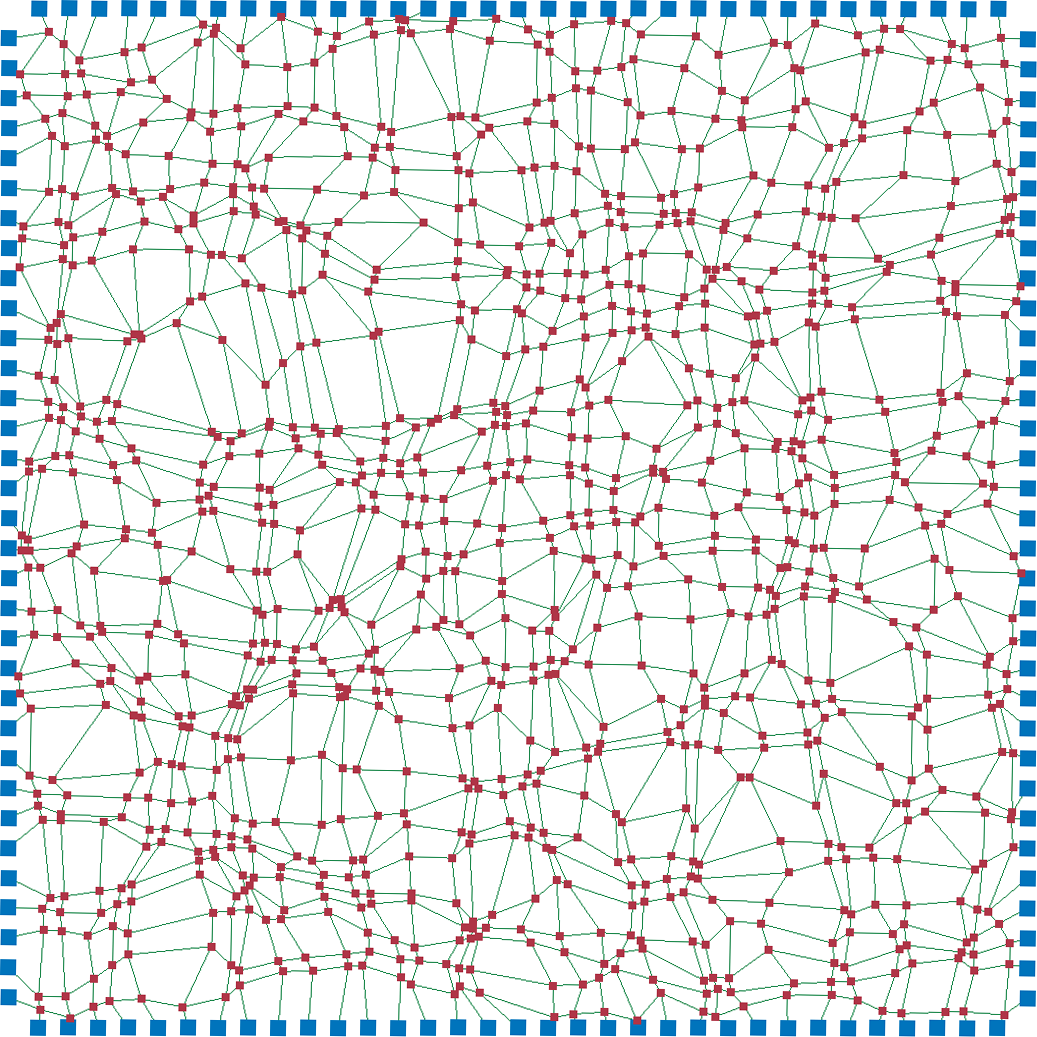
\includegraphics[
		width=\textwidth, 
		height=\textwidth, 
		keepaspectratio=true]
	{./img/results/1200_0_1_stretchGreaterThan_104_step_3}
	%\caption{Step 2}
	%\label{fig:experiment:stretchGreaterThanStrain:3}
\end{subfigure}			
\begin{subfigure}{0.16\textwidth}
	\centering
	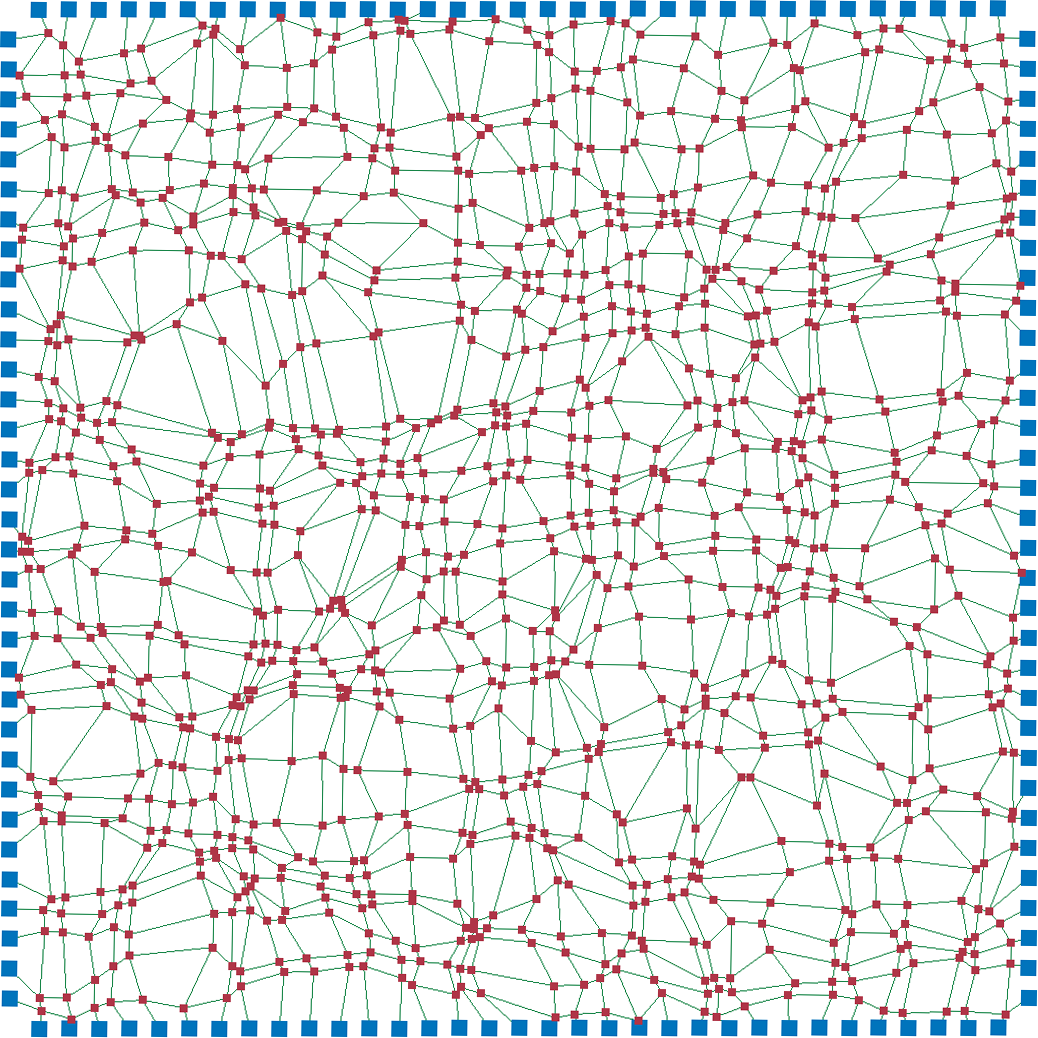
\includegraphics[
		width=\textwidth, 
		height=\textwidth, 
		keepaspectratio=true]
	{./img/results/1200_0_1_stretchGreaterThan_104_step_4}
	%\caption{Step 3}
	%\label{fig:experiment:stretchGreaterThanStrain:4}
\end{subfigure}				
\begin{subfigure}{0.16\textwidth}
	\centering
	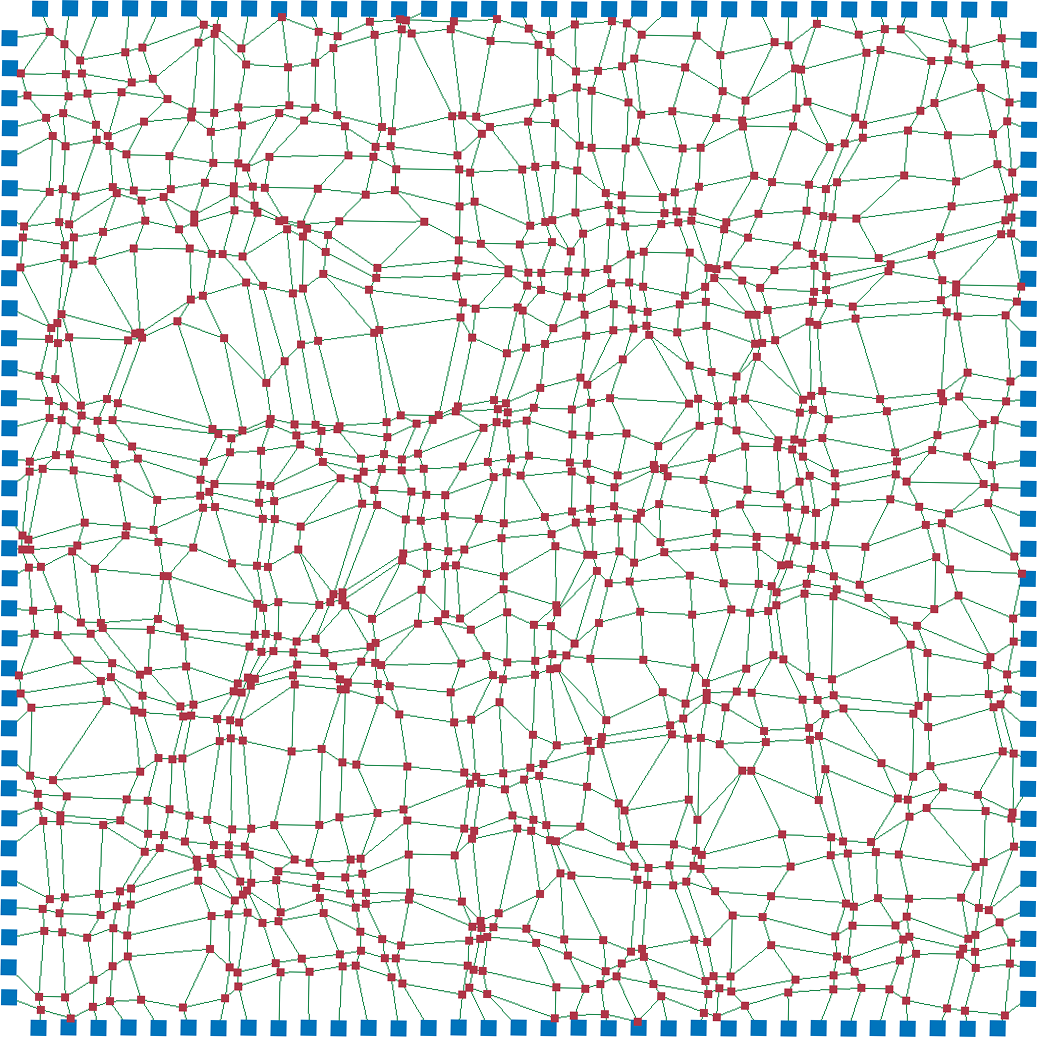
\includegraphics[
		width=\textwidth, 
		height=\textwidth, 
		keepaspectratio=true]
	{./img/results/1200_0_1_stretchGreaterThan_104_step_5}
	%\caption{Step 4}
	%\label{fig:experiment:stretchGreaterThanStrain:5}
\end{subfigure}					
	\caption{Several steps of the stretching of springs, $\vartheta = 0.1$, where the springs with a strain greater than 1.04 were stretched. The grid had 1200 particles, the spring constants were sampled from a normal distribution with mean 0.0 and standard deviation 1.0. Step 0 is a stabilization of the initial grid, presented in \cref{fig:implementation:stabilizedInitial}, the following steps are the stabilization and breaking steps of the algorithm.}
	\label{fig:experiment:stretchGreaterThanStrain}
\end{figure*}

\begin{figure*}
	\centering
	%!TEX root = report.tex	
\begin{subfigure}{0.16\textwidth}
	\centering
	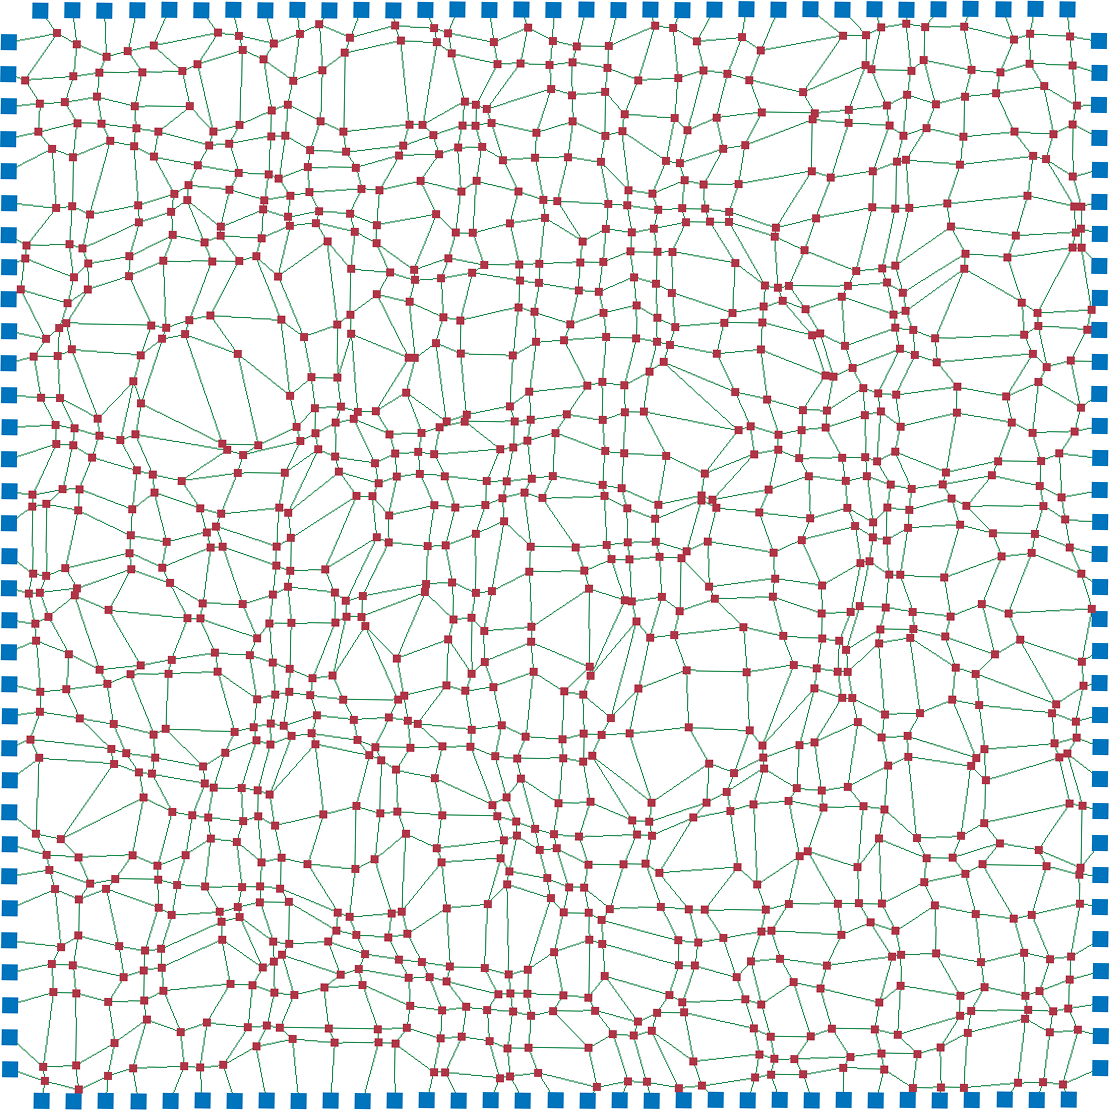
\includegraphics[
		width=\textwidth, 
		height=\textwidth, 
		keepaspectratio=true]
	{./img/results/1200_0_1_stretchHighest_97_step_0}
	\caption{Step 0}
	\label{fig:experiment:stretchHighestStrain:0}
\end{subfigure}	
\begin{subfigure}{0.16\textwidth}
	\centering
	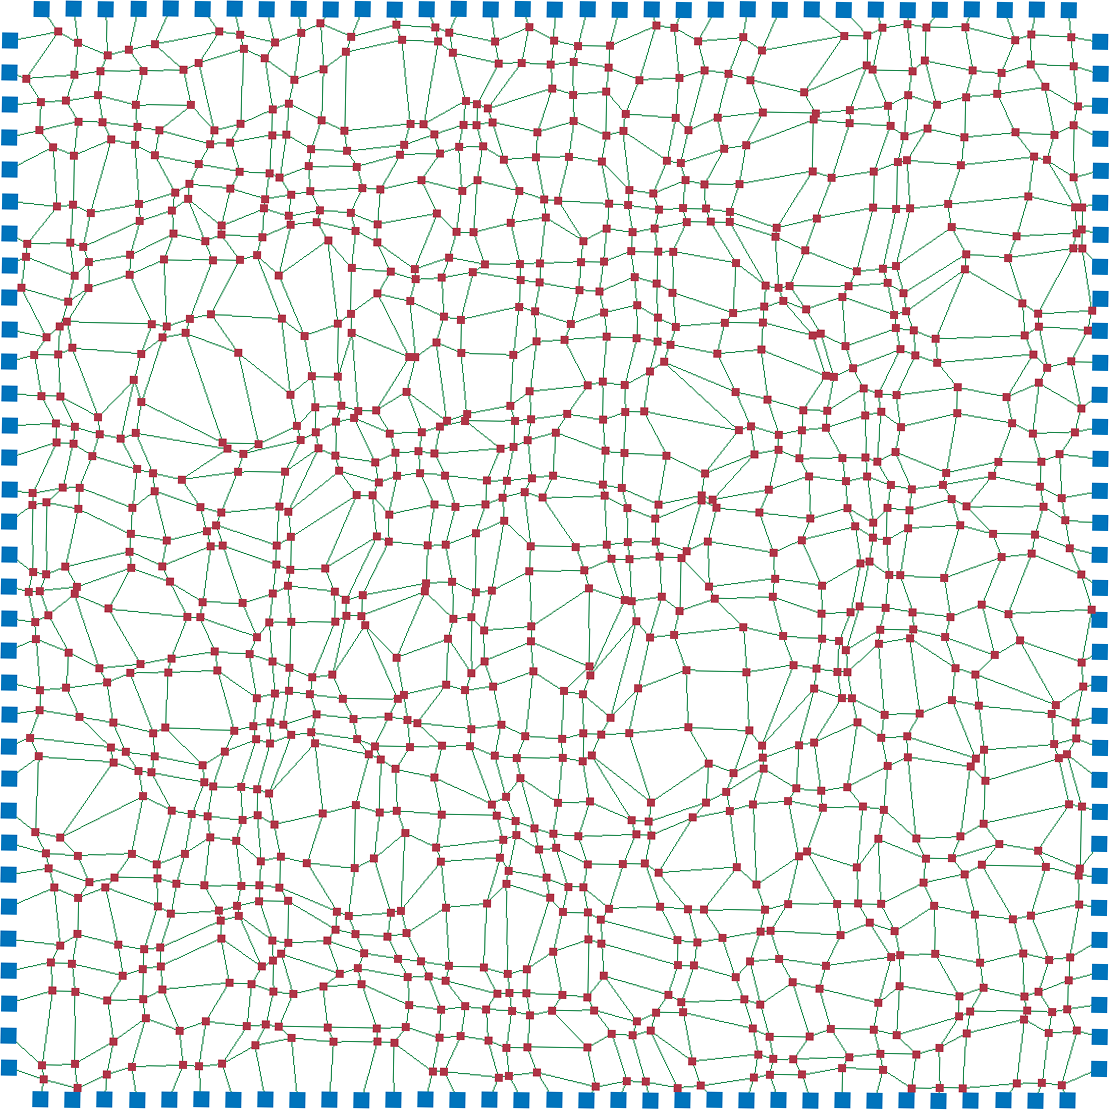
\includegraphics[
		width=\textwidth, 
		height=\textwidth, 
		keepaspectratio=true]
	{./img/results/1200_0_1_stretchHighest_97_step_1}
	\caption{Step 1}
	\label{fig:experiment:stretchHighestStrain:1}
\end{subfigure}		
\begin{subfigure}{0.16\textwidth}
	\centering
	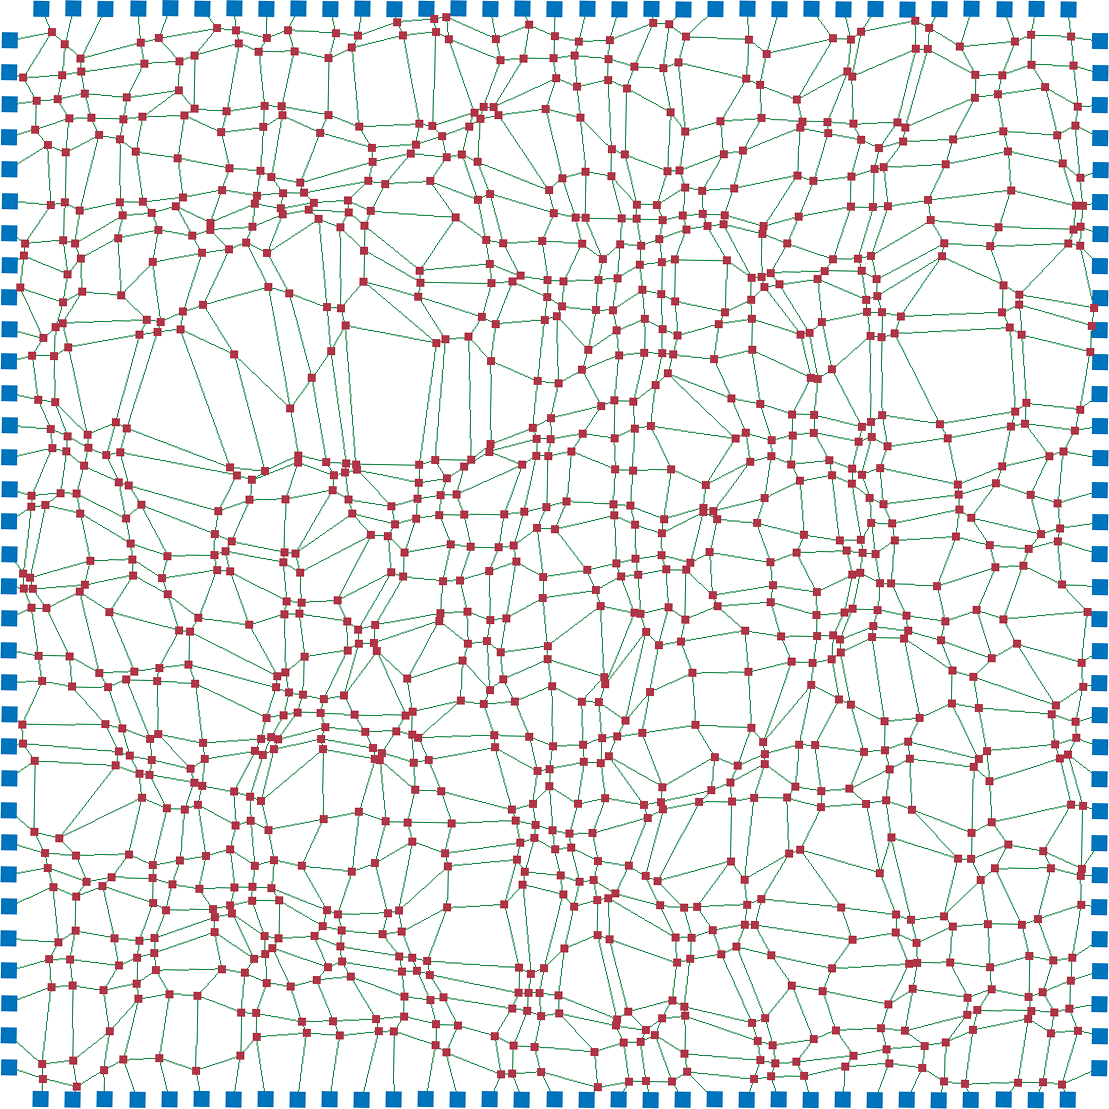
\includegraphics[
		width=\textwidth, 
		height=\textwidth, 
		keepaspectratio=true]
	{./img/results/1200_0_1_stretchHighest_97_step_2}
	\caption{Step 2}
	\label{fig:experiment:stretchHighestStrain:2}
\end{subfigure}			
\begin{subfigure}{0.16\textwidth}
	\centering
	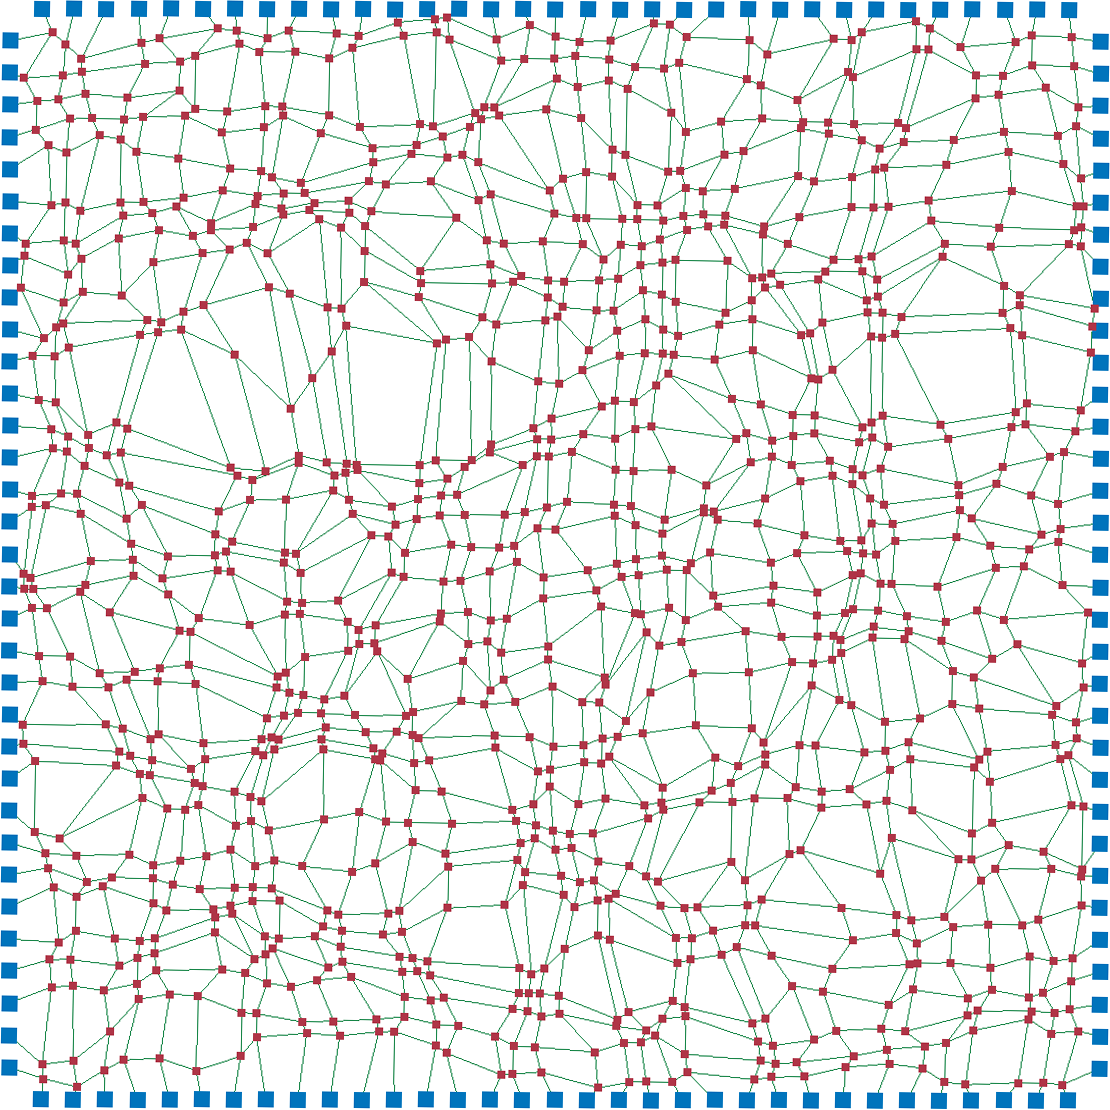
\includegraphics[
		width=\textwidth, 
		height=\textwidth, 
		keepaspectratio=true]
	{./img/results/1200_0_1_stretchHighest_97_step_3}
	\caption{Step 3}
	\label{fig:experiment:stretchHighestStrain:3}
\end{subfigure}				
\begin{subfigure}{0.16\textwidth}
	\centering
	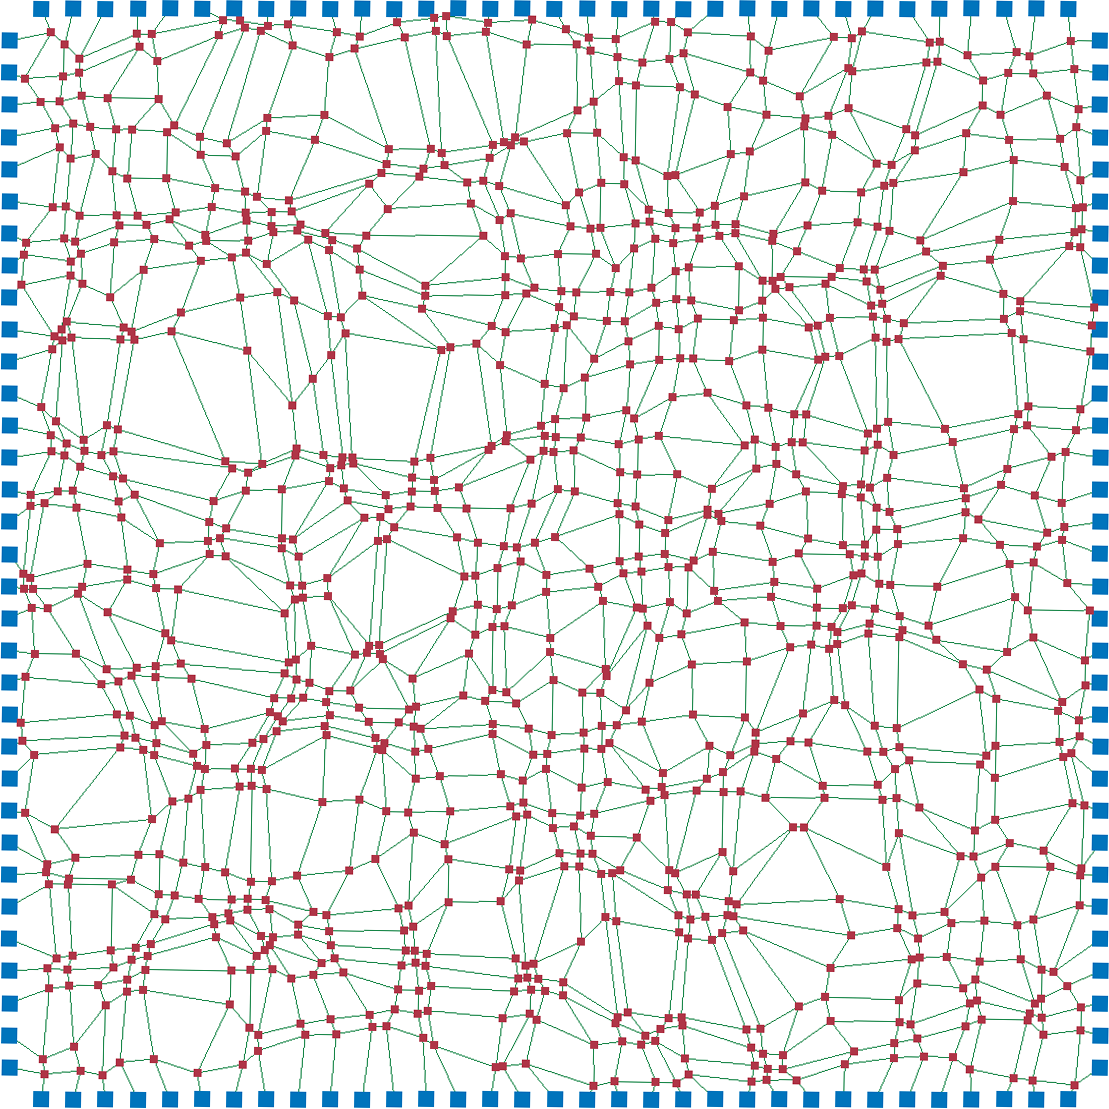
\includegraphics[
		width=\textwidth, 
		height=\textwidth, 
		keepaspectratio=true]
	{./img/results/1200_0_1_stretchHighest_97_step_4}
	\caption{Step 4}
	\label{fig:experiment:stretchHighestStrain:4}
\end{subfigure}
\begin{subfigure}{0.16\textwidth}
	\centering
	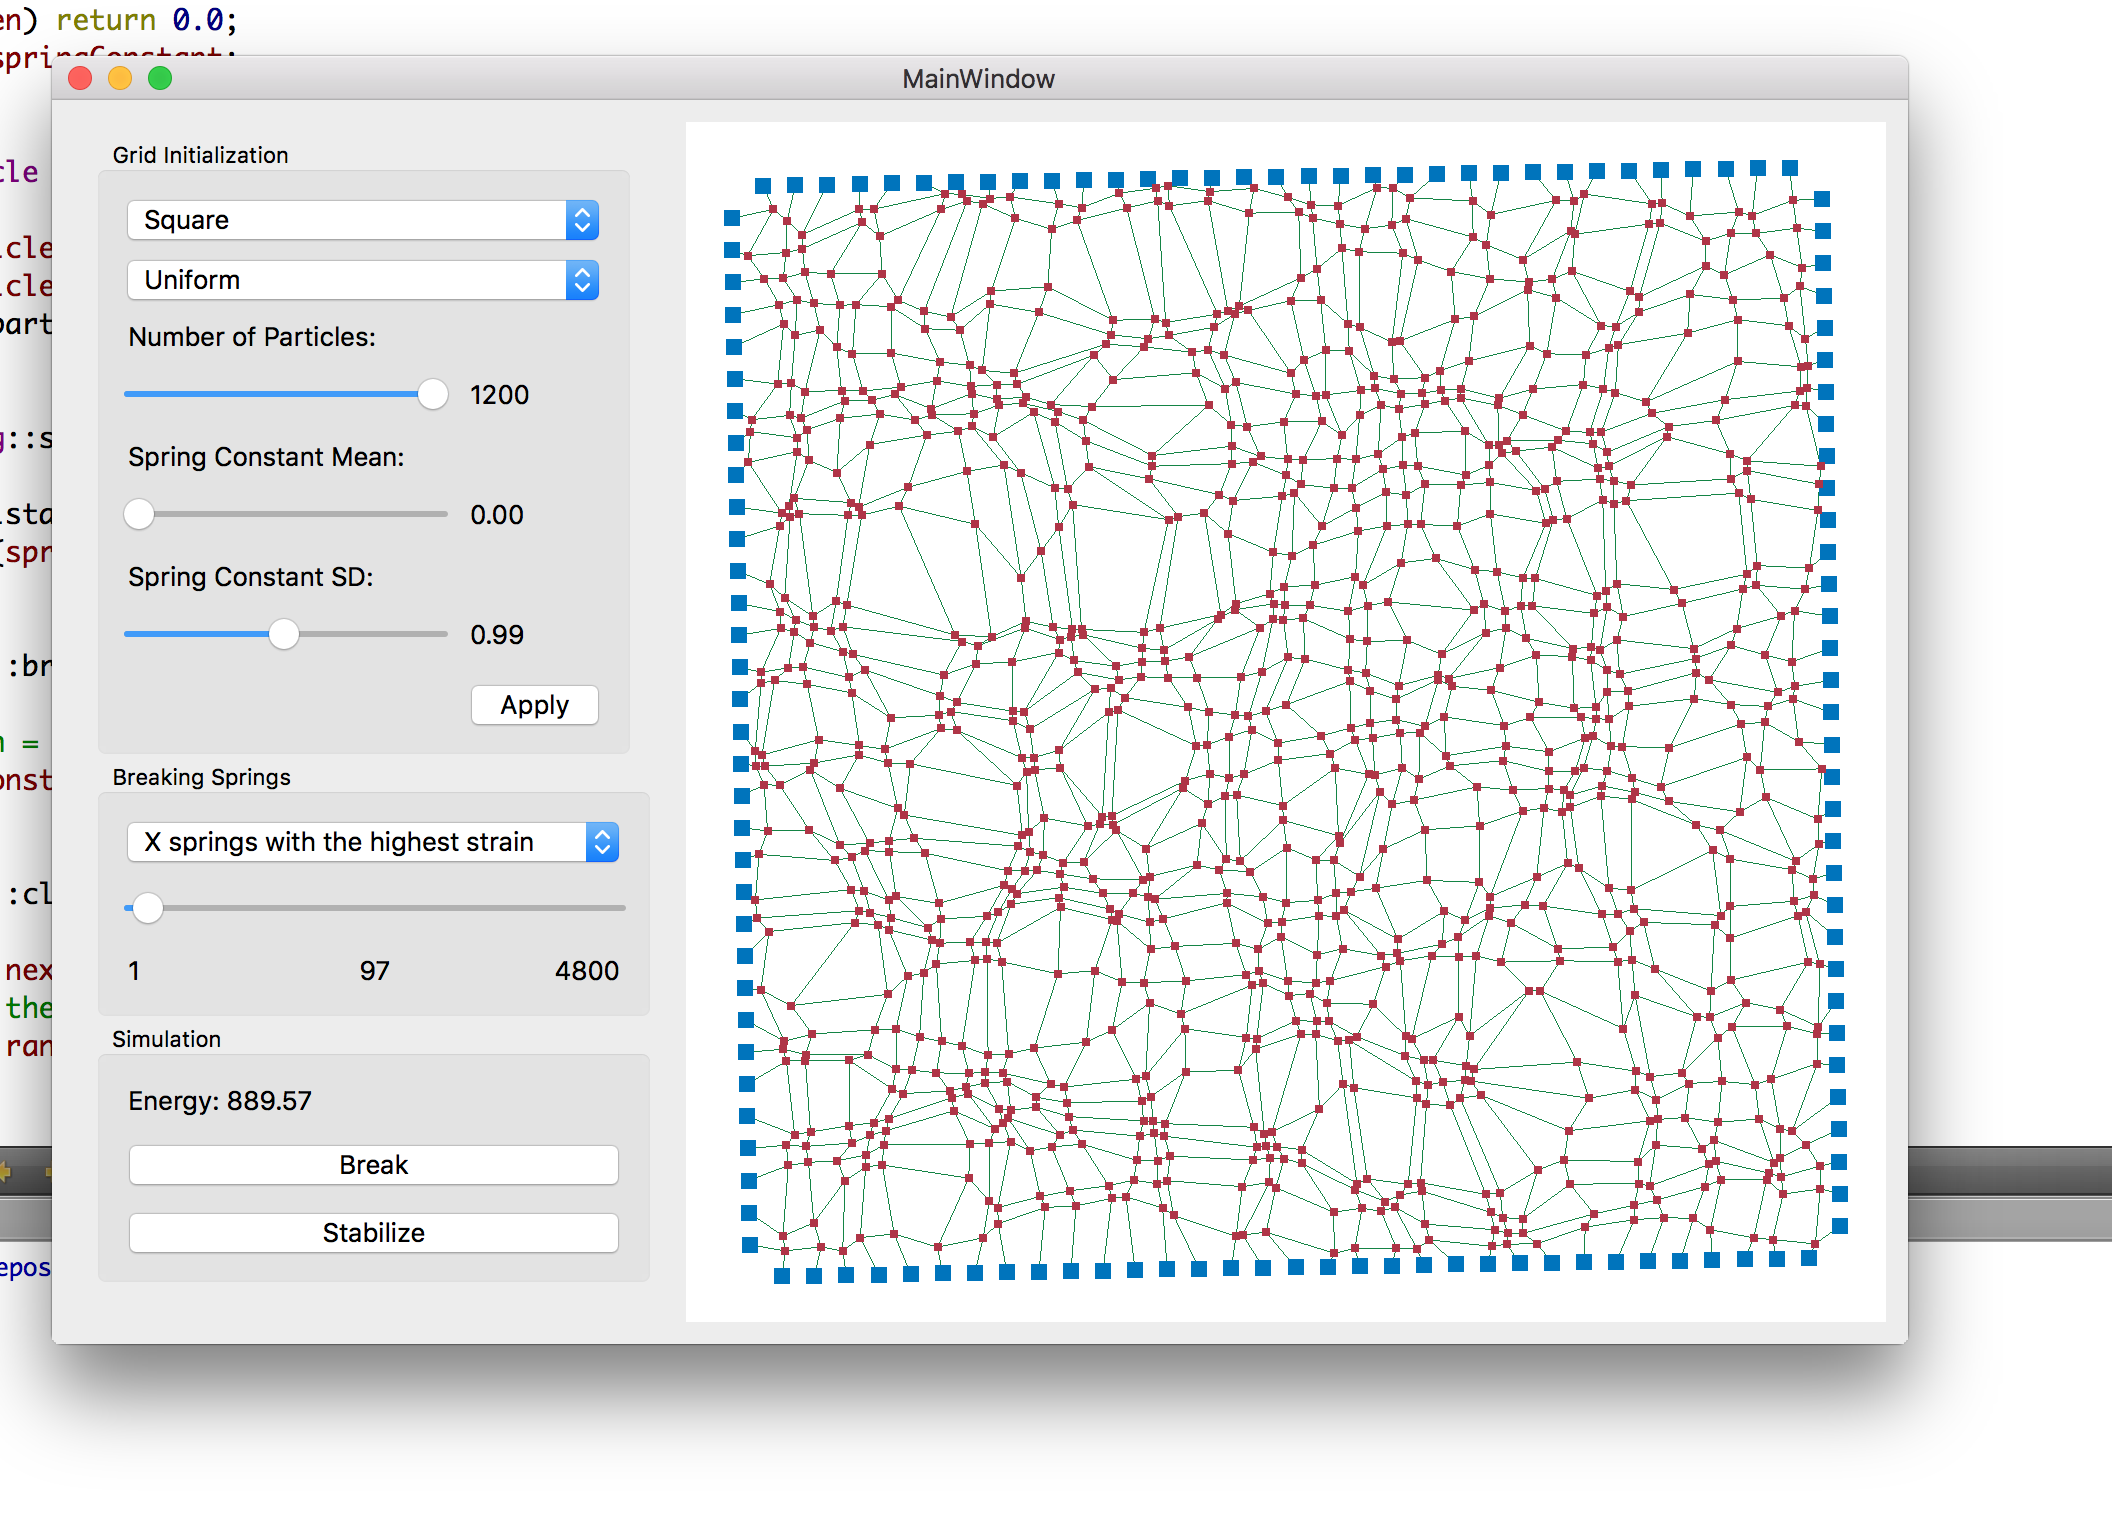
\includegraphics[
		width=\textwidth, 
		height=\textwidth, 
		keepaspectratio=true]
	{./img/results/1200_0_1_stretchHighest_97_step_5}
	\caption{Step 4}
	\label{fig:experiment:stretchHighestStrain:5}
\end{subfigure}

\begin{subfigure}{0.16\textwidth}
	\centering
	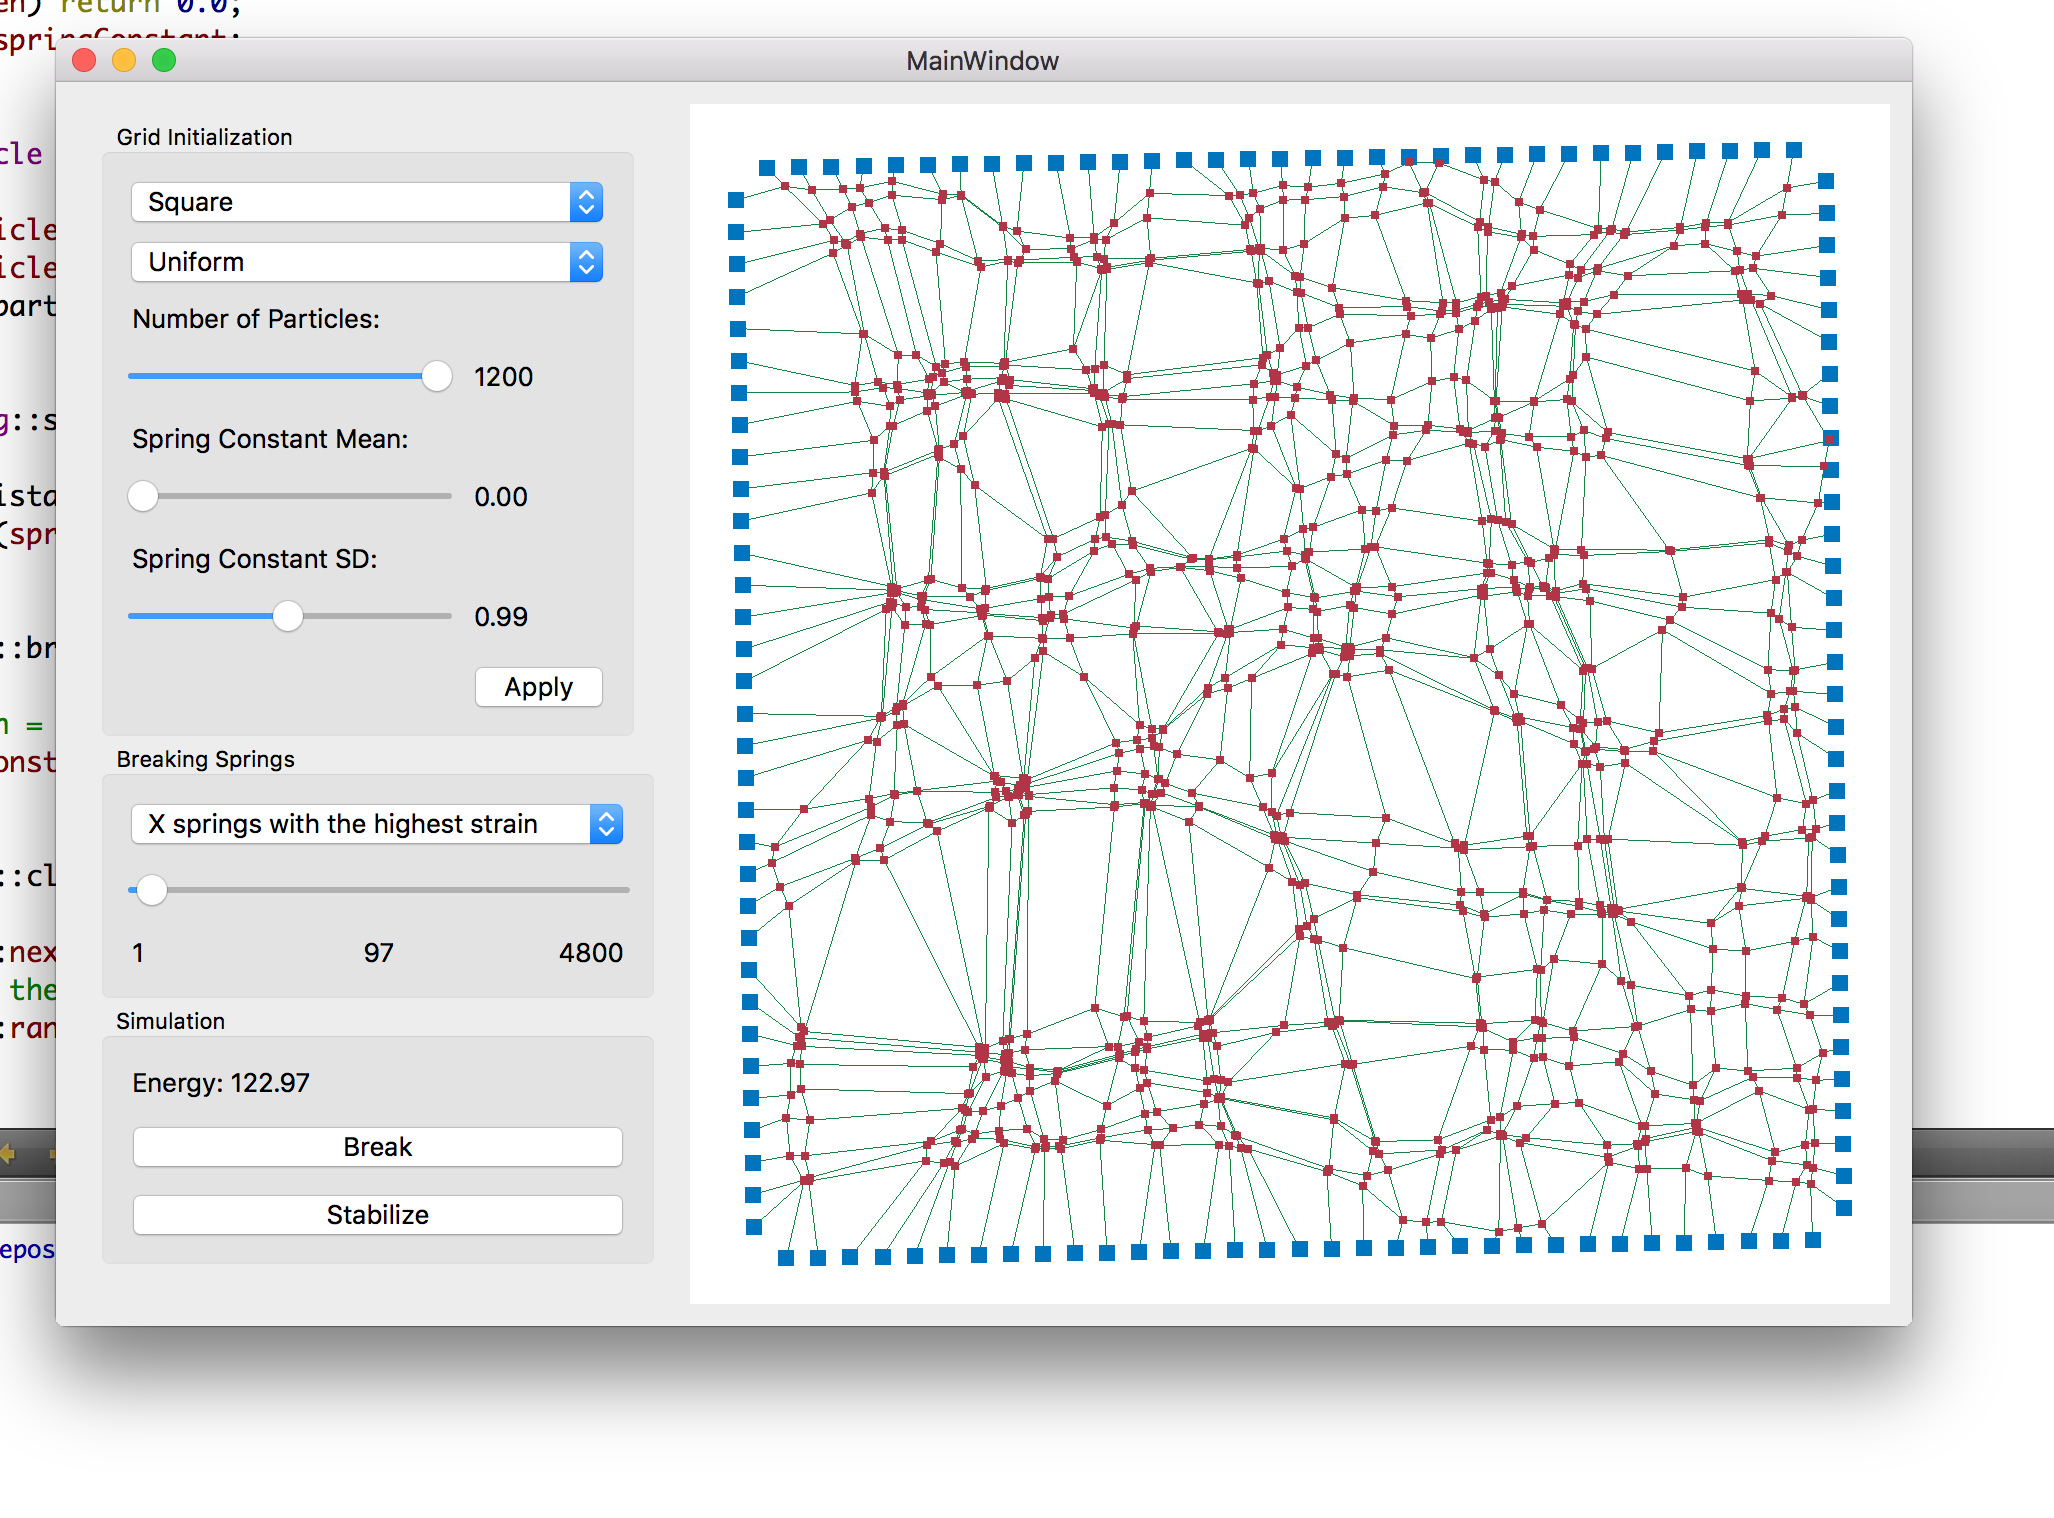
\includegraphics[
		width=\textwidth, 
		height=\textwidth, 
		keepaspectratio=true]
	{./img/results/1200_0_1_stretchHighest_97_step_50}
	\caption{Step 50}
	\label{fig:expe riment:stretchHighestStrain:50}
\end{subfigure}	
\begin{subfigure}{0.16\textwidth}
	\centering
	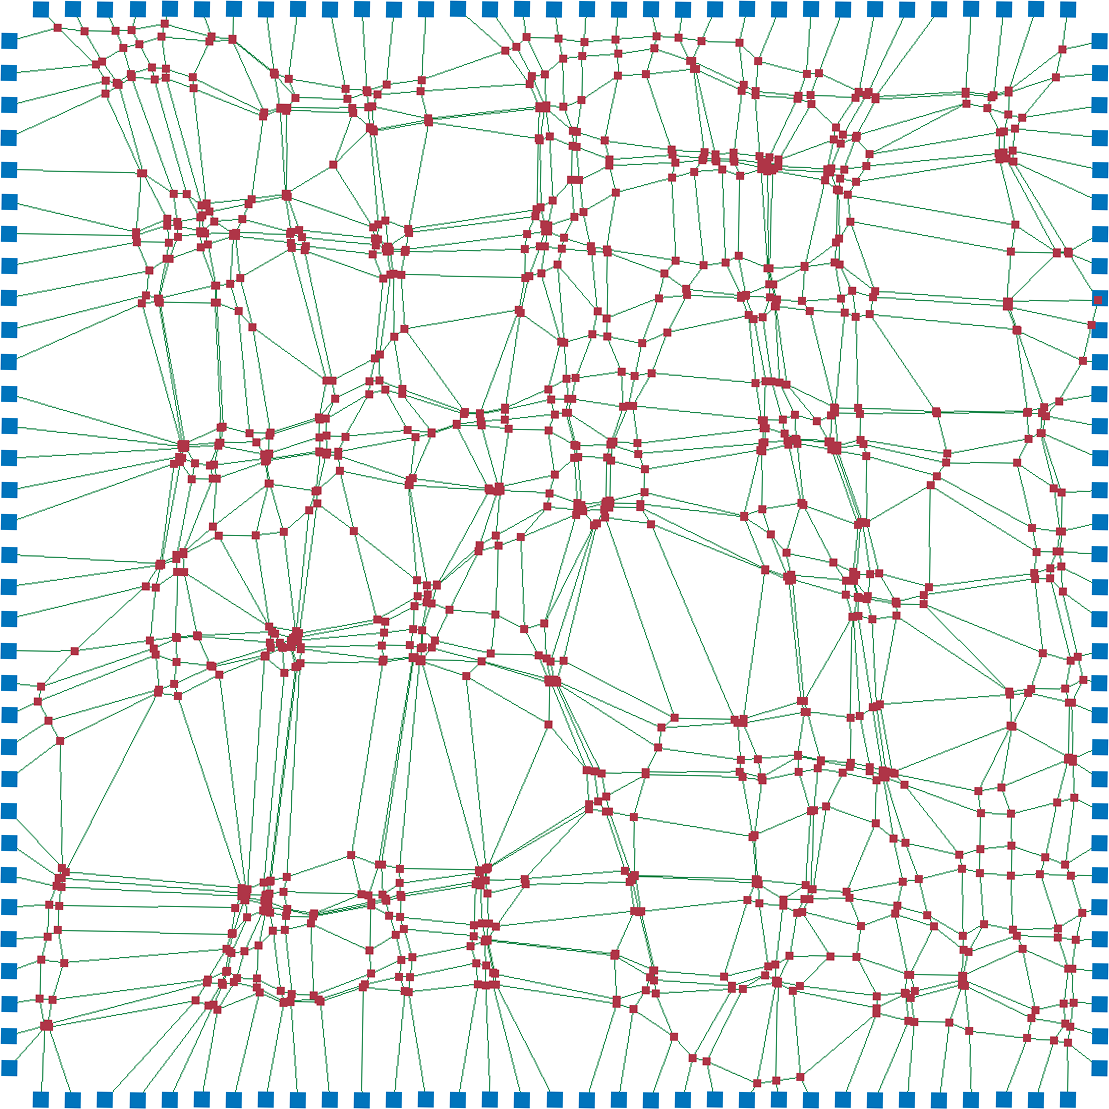
\includegraphics[
		width=\textwidth, 
		height=\textwidth, 
		keepaspectratio=true]
	{./img/results/1200_0_1_stretchHighest_97_step_51}
	\caption{Step 51}
	\label{fig:experiment:stretchHighestStrain:51}
\end{subfigure}		
\begin{subfigure}{0.16\textwidth}
	\centering
	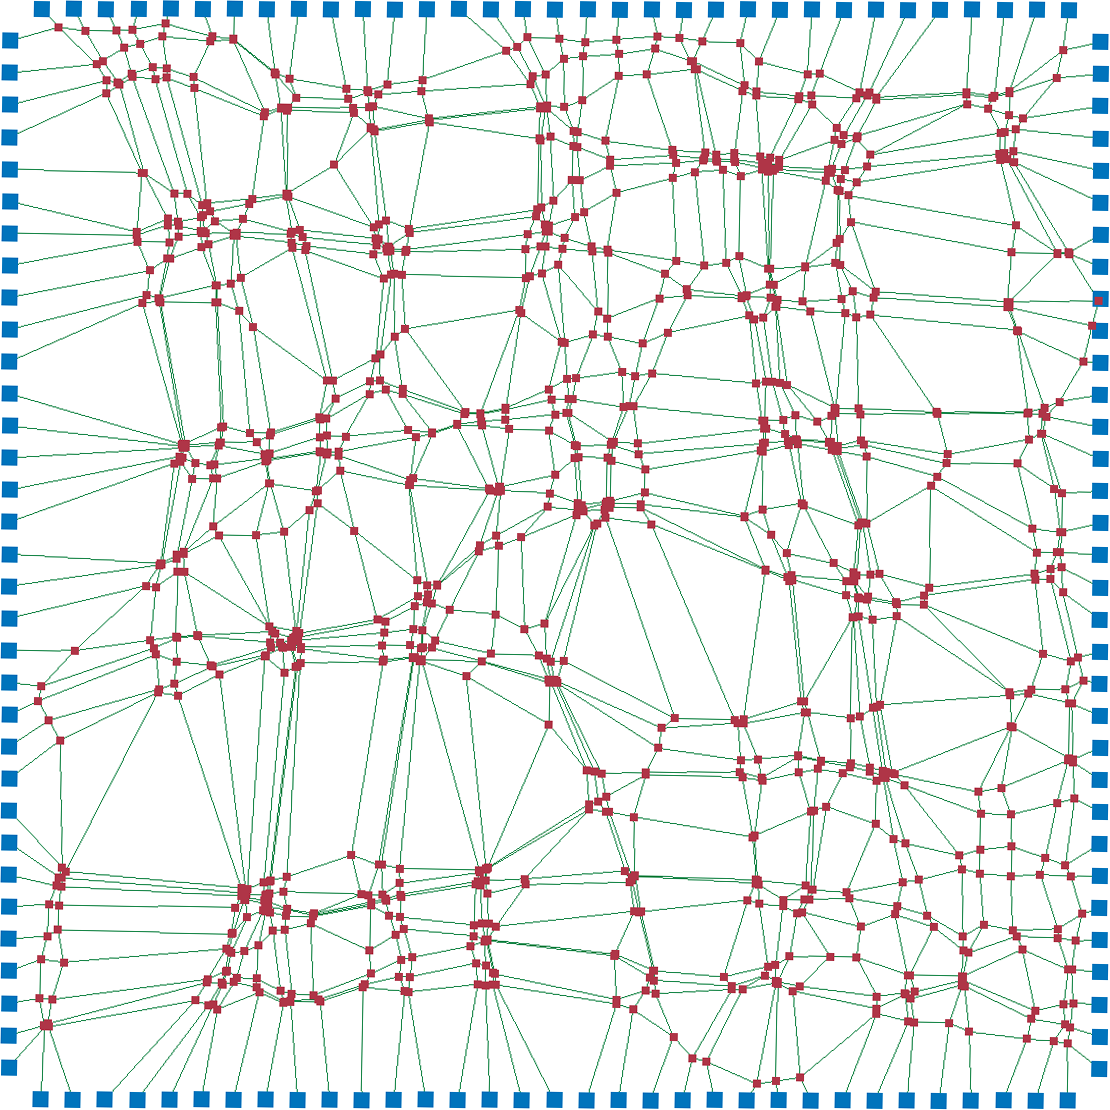
\includegraphics[
		width=\textwidth, 
		height=\textwidth, 
		keepaspectratio=true]
	{./img/results/1200_0_1_stretchHighest_97_step_52}
	\caption{Step 52}
	\label{fig:experiment:stretchHighestStrain:52}
\end{subfigure}			
\begin{subfigure}{0.16\textwidth}
	\centering
	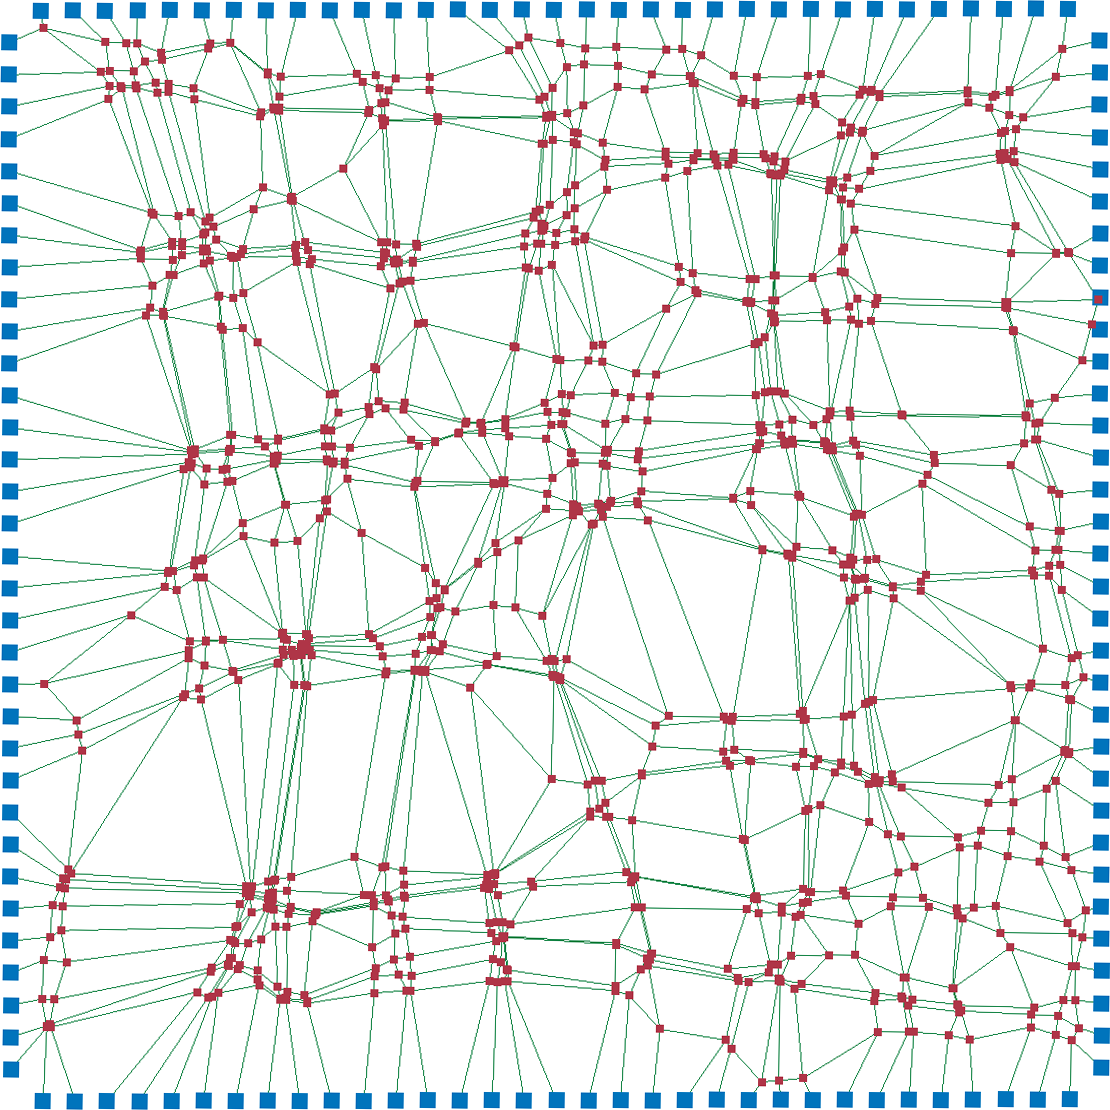
\includegraphics[
		width=\textwidth, 
		height=\textwidth, 
		keepaspectratio=true]
	{./img/results/1200_0_1_stretchHighest_97_step_53}
	\caption{Step 53}
	\label{fig:experiment:stretchHighestStrain:53}
\end{subfigure}				
\begin{subfigure}{0.16\textwidth}
	\centering
	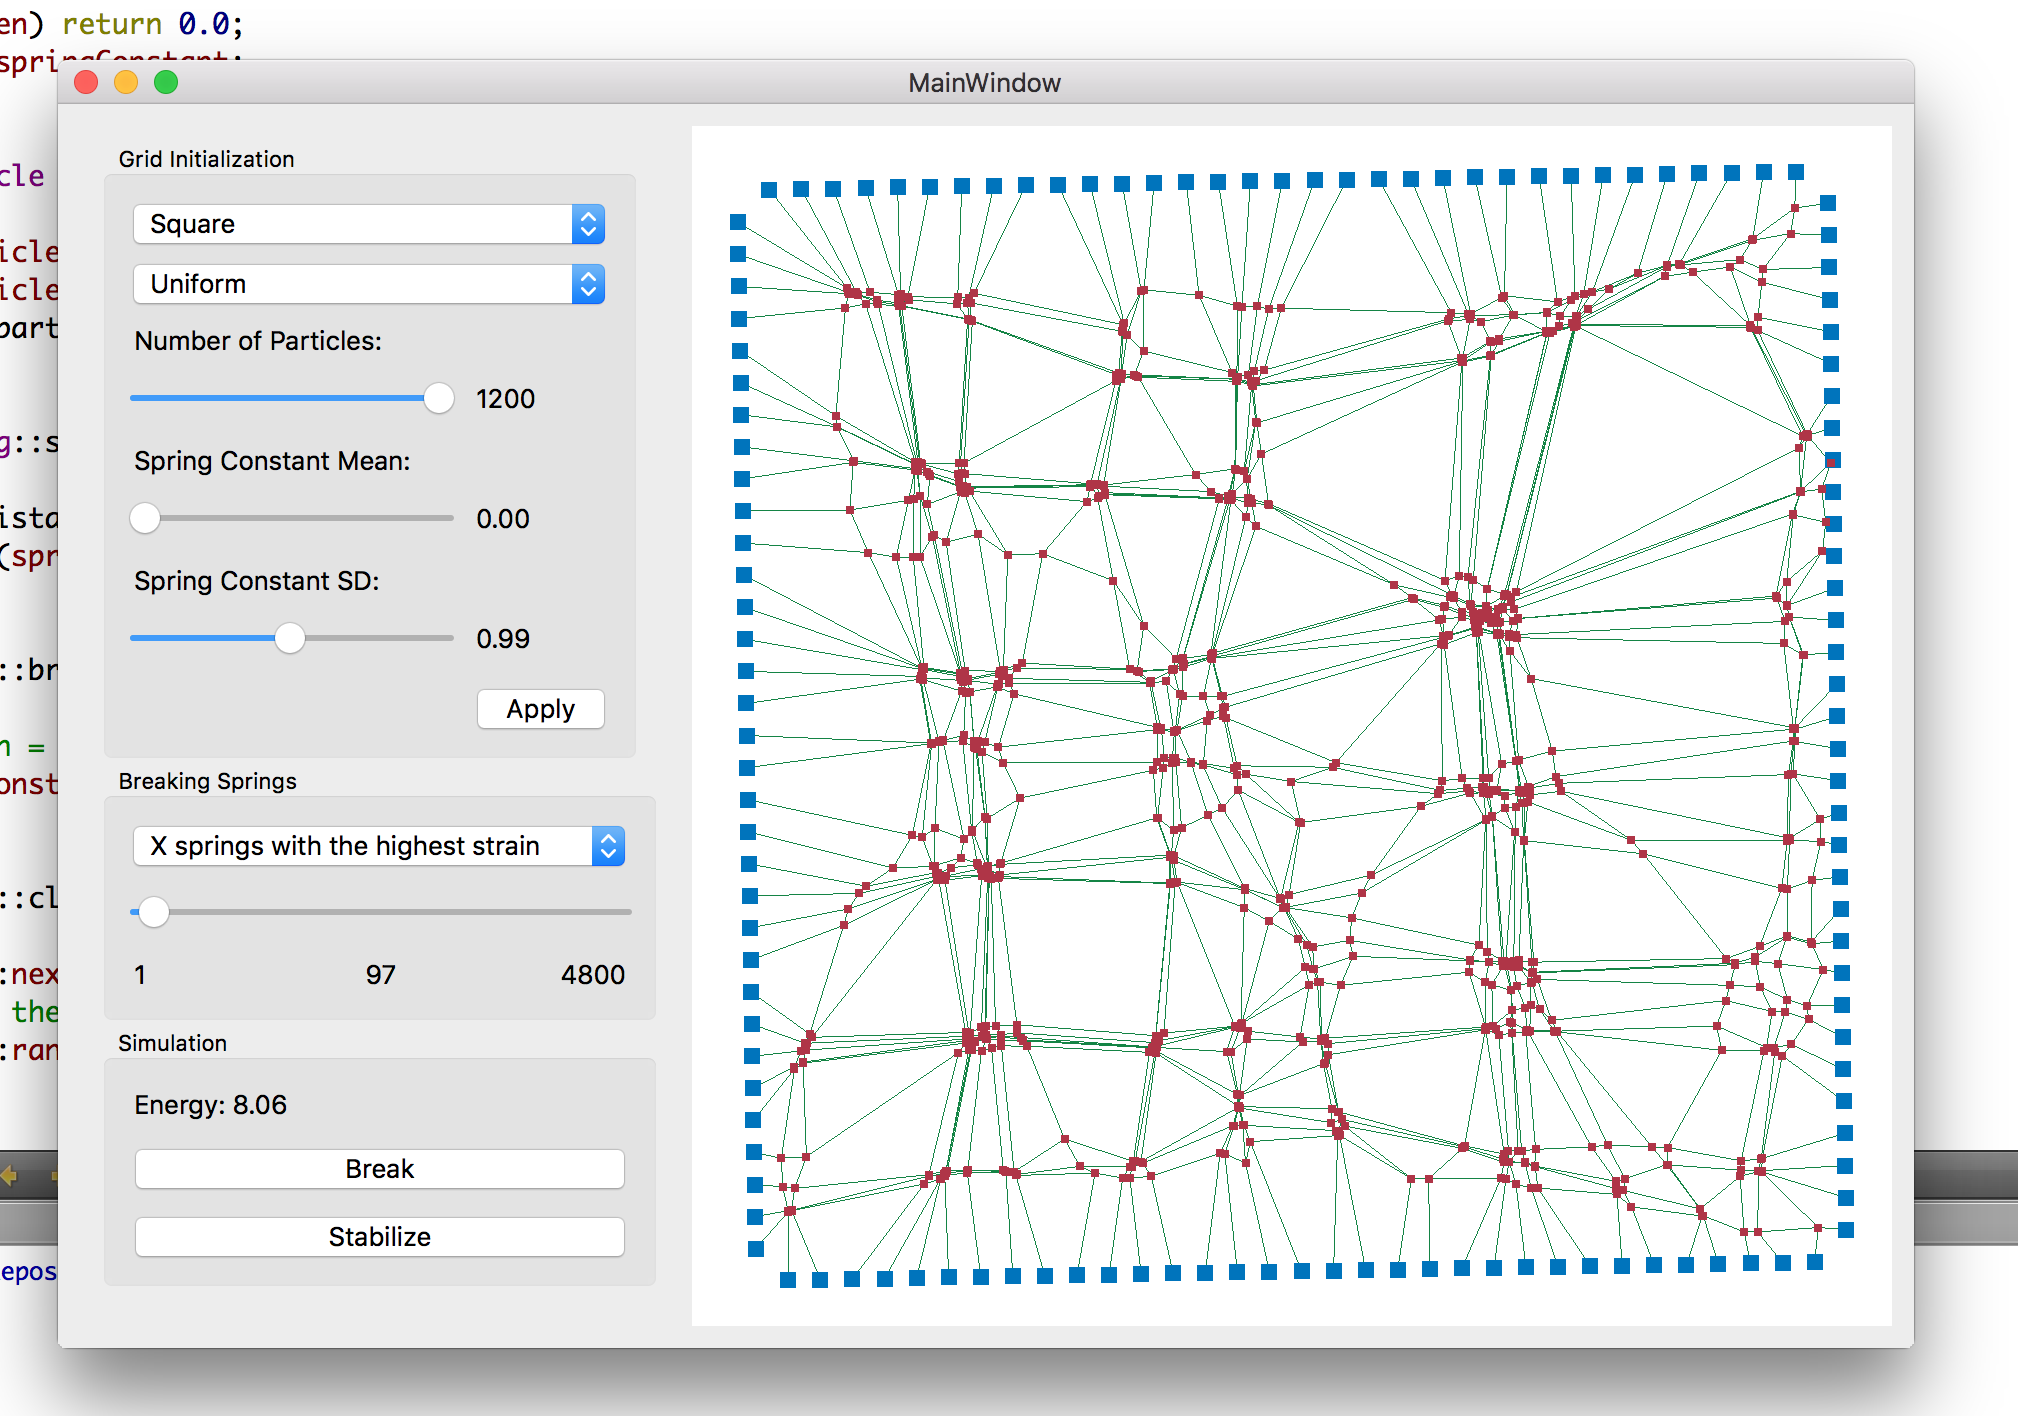
\includegraphics[
		width=\textwidth, 
		height=\textwidth, 
		keepaspectratio=true]
	{./img/results/1200_0_1_stretchHighest_97_step_80}
	\caption{Step 80}
	\label{fig:experiment:stretchHighestStrain:80}
\end{subfigure}
\begin{subfigure}{0.16\textwidth}
	\centering
	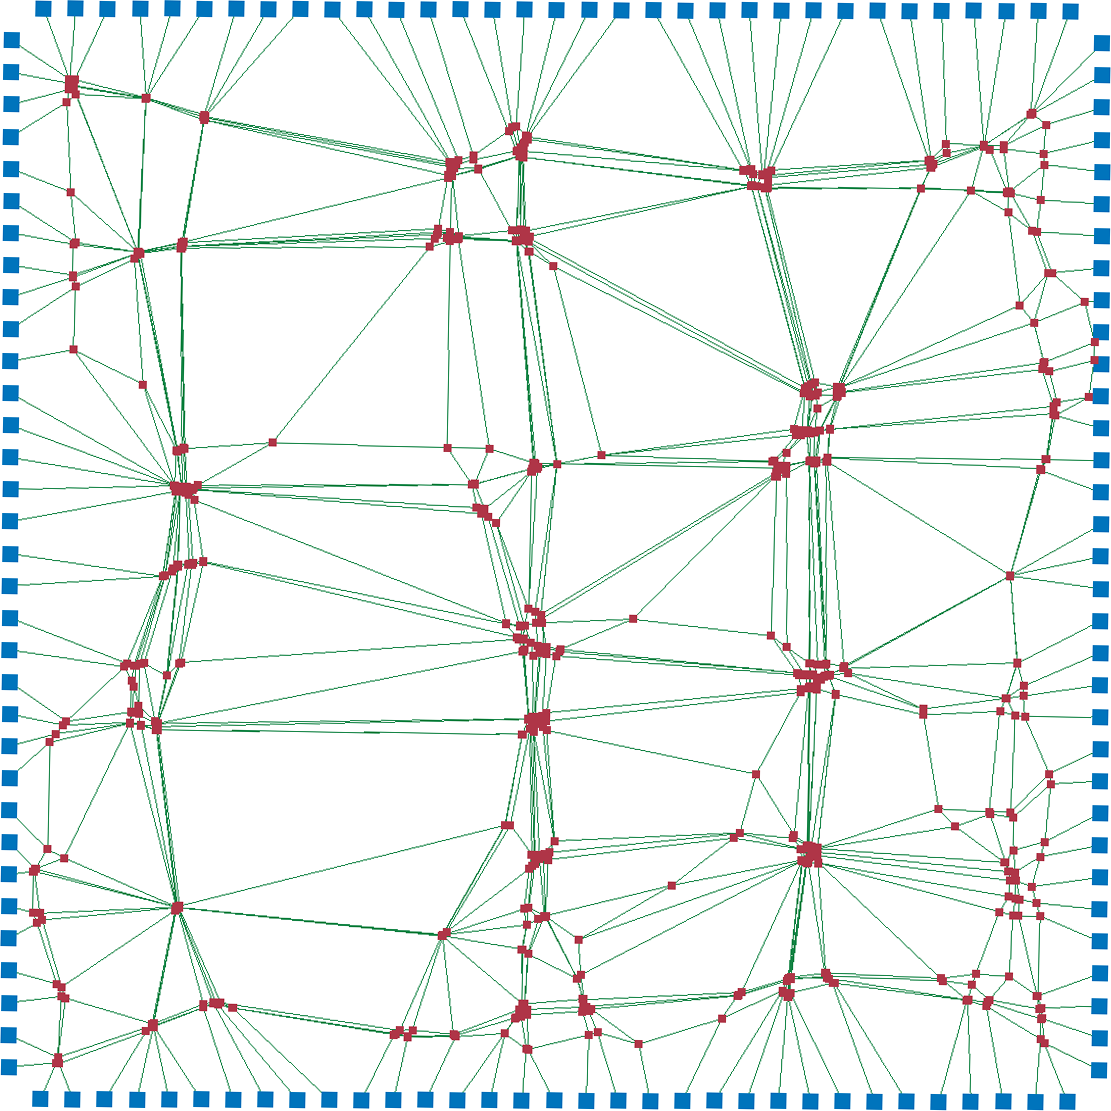
\includegraphics[
		width=\textwidth, 
		height=\textwidth, 
		keepaspectratio=true]
	{./img/results/1200_0_1_stretchHighest_97_step_100}
	\caption{Step 100}
	\label{fig:experiment:stretchHighestStrain:100}
\end{subfigure}					
	\caption{Several steps of the stretching of springs, $\vartheta = 0.1$, where the 97 springs with the highest strain were stretched. The grid had 1200 particles, the spring constants were sampled from a normal distribution with mean 0.0 and standard deviation 1.0. Step 0 is a stabilization of the initial grid, presented in \cref{fig:implementation:stabilizedInitial}, the following steps are the stabilization and breaking steps of the algorithm.}
	\label{fig:experiment:stretchHighest}
\end{figure*}